% fable_cosmology.tex -- fableScalar and fable on the 4+4 pre-universe: the paper of fable-cosmology/.
% Build (MiKTeX or TeX Live), from this directory:
%     latexmk -pdf -interaction=nonstopmode -halt-on-error fable_cosmology.tex
% Every number in this paper is read from a file of the repository (fable-cosmology/results/*.csv,
% fable-cosmology/reference/*.csv, the executed notebooks, claude-fable/run_fable51_part6.log);
% the figures are the PNGs the notebooks write to fable-cosmology/results/, copied to figures/.
\documentclass[11pt,a4paper]{article}

\usepackage[T1]{fontenc}
\usepackage[utf8]{inputenc}
\usepackage{lmodern}
\usepackage[margin=2.5cm]{geometry}
\usepackage{microtype}
\usepackage{amsmath,amssymb}
\usepackage{graphicx}
\usepackage{booktabs}
\usepackage{tabularx}
\usepackage{caption}
\usepackage{subcaption}
\usepackage{placeins}
\usepackage{enumitem}
\usepackage{fancyvrb}
\usepackage{upquote}
\usepackage[hidelinks]{hyperref}

\graphicspath{{figures/}}
\captionsetup{font=small,labelfont=bf}
\setlist{itemsep=2pt,topsep=4pt}
\fvset{fontsize=\footnotesize,xleftmargin=1em}
\newcolumntype{Y}{>{\raggedright\arraybackslash}X}

\newcommand{\fableScalar}{\textsf{fableScalar}}
\newcommand{\fable}{\textsf{fable}}
\newcommand{\Lhat}{\hat{L}}
\newcommand{\sig}{\sigma_{16}}
\newcommand{\T}[1]{T_{16}[#1]}
\newcommand{\sgn}{\sqrt{g}}
\newcommand{\dd}{\mathrm{d}}
\newcommand{\diag}{\operatorname{diag}}
\newcommand{\Hobs}{H_{\mathrm{obs}}}
\newcommand{\Vhid}{\mathcal{V}_{\mathrm{hid}}}
\newcommand{\file}[1]{\path{#1}}
\pdfstringdefDisableCommands{\def\fableScalar{fableScalar}\def\fable{fable}}

\title{\fableScalar{} and \fable{}: a quintessence-like scalar and a 16-component spinor on the
4+4 pre-universe, their equations of state, and the Supernovae \emph{Unite} CPL fits}
\author{Prepared with Claude (Anthropic) at the direction of Patrick L.~Nash\thanks{The 4+4
pre-universe, its frame field and the Lagrangian of the 16-component spinor are the work of
Patrick L.~Nash, Ph.D.\ (\copyright~2022, GNU General Public License), refactored and extended in
the repository that contains this paper. The fields, the solver, the notebooks and this paper
were prepared with Claude (Anthropic) at his direction on 2026-09-16 and completed on
2026-09-24.}}
\date{2026-09-24}

\begin{document}
\maketitle

\begin{abstract}
We define two fields on the 4+4-dimensional pre-universe of P.~L.~Nash: \fableScalar{}, a
minimally coupled real scalar $\phi$ with self-interaction $V(\phi)$, and \fable{}, a real
16-component $\mathrm{Spin}(4,4)$ spinor $\Psi$ with self-interaction $V(s)$ of its scalar bilinear
$s=\Psi^{T}\sig\Psi$. For each we derive, and verify symbolically in Mathematica (358 of 358
assertions pass), the Lagrangian, the energy--momentum tensor, the field equation, the kinetic
and potential energies, the energy density $\rho$, the pressure $P$ and the equation of state
$w=P/\rho$, and we integrate the resulting cosmologies with the pure-Rust translation of
SUNDIALS~7.8.0 CVODE taken from the author's rustSolveIt repositories. On the pre-universe the
8-volume element does not depend on the observer's time, so there is no Hubble friction: a
homogeneous \fableScalar{} oscillates undamped with the virial average
$\langle w\rangle=(n-1)/(n+1)$ for $V\propto\phi^{2n}$ (measured $+0.0044$ and $+0.3349$ over 100
time units for $n=1,2$); a static profile along the hidden coordinate is $w=-1$ on the observed
sheet; and the bilinear of \fable{} does not dilute at all. The null energy condition
$\rho+P=2\,\mathrm{KE}$ holds identically for \fableScalar{}, so $w_\phi\ge-1$ wherever
$\rho_\phi>0$. For \fable{} on its homogeneous solutions $w=sV'(s)/V(s)-1$: the author's own mass
term is exactly pressureless dust, and a potential whose slope changes sign carries $w$ across
$-1$ with no wrong-sign kinetic term. In the 4-dimensional reference models (a Friedmann
equation on a separate FLRW frame) a thawing exponential \fableScalar{} has the sign pattern of the
Supernovae \emph{Unite} CPL fit $(w_0,w_a)=(-0.861,-0.60)$ but never both numbers (closest,
$\lambda=1.4$: $(-0.674,-0.435)$), while a \fable{} spinor with $V=V_0+m\,s\,e^{-s/s_1}$ reproduces
them to a few hundredths ($(-0.851,-0.569)$, distance $0.032$) with a genuine phantom phase in the
past (minimum $w=-1.388$) and $\rho>0$ throughout. CVODE, scipy's DOP853 and Mathematica's
\texttt{NDSolve} agree to $1.3\times10^{-10}$ (scalar) and $1.9\times10^{-8}$ (spinor) in $w$. The
framework has no gravitational sector, so which density gravitates, and the value of the
scale-factor function $a_4$, remain undetermined.
\end{abstract}

\tableofcontents

% =====================================================================================
\section{Introduction}\label{sec:intro}

The task set by the author was to define a scalar field, \fableScalar{}, and a 16-component
spinor field, \fable{}, each inspired by quintessence, each filling the pre-universe and evolving
in time, each providing a physical mechanism for a time-varying equation of state of dark energy;
to define, verify and test their Lagrangians and energy--momentum tensors, their kinetic and
potential energies, pressures, energy densities and equations of state; to investigate the
behaviour of $w$ with numerical solutions and graphs; and to answer whether there is a connection
to dark matter or dark energy.

The observational reference is the author's note of 2026-09-15 (unpublished; its content is
restated here). It uses the Chevallier--Polarski--Linder (CPL) parameterisation
\cite{Chevallier2001,Linder2003}
\begin{equation}\label{eq:cpl}
  w(a)=w_0+w_a(1-a),
\end{equation}
and two fits to the Supernovae \emph{Unite} data: forcing a constant equation of state gives
$w=-0.764$, two standard deviations from $-1$; letting it vary gives
$(w_0,w_a)=(-0.861,-0.60)$. The CPL line of the second fit reaches $-0.861$ today, crosses $-1$ at
$a=1-0.139/0.60=0.768$ and extrapolates to $w_0+w_a=-1.461$ as $a\to0$. The ``phantom past'' of
that line lies at $a\lesssim0.77$ and, below $a\approx0.3$, outside the supernova range: it is an
extrapolation of a straight line, not a measurement of $w<-1$. The note also recalls canonical
quintessence \cite{Ratra1988,Wetterich1988,Caldwell1998}, $L=\tfrac12\partial\phi\partial\phi-V$,
$\rho=\tfrac12\dot\phi^2+V$, $P=\tfrac12\dot\phi^2-V$, $\ddot\phi+3H\dot\phi+V'=0$; the distinction
between thawing and freezing fields \cite{Caldwell2005}; and the fact that a canonical scalar
cannot cross the phantom divide $w=-1$ \cite{Caldwell2002,Vikman2005}.

Two kinds of statement are made in this paper and they are kept apart throughout. The first kind
is \emph{exact on the 8-dimensional pre-universe}: definitions, tensors, field equations and their
consequences, each proved symbolically in Part~VI of the Mathematica notebook
\file{claude-fable/claude-fable_Einstein-Rosen-2-Planes.nb} (Sections~23--25). The second kind
belongs to \emph{4-dimensional reference models}: a Friedmann equation on a separate FLRW frame,
which the pre-universe does not supply (it has no gravitational sector and its scale-factor
function $a_4$ is undetermined), used because it is the standard setting of the CPL fits. The
reference models are never substituted into the pre-universe frame and never give $a_4$ a value.

Section~\ref{sec:frame} recalls the geometry; Sections~\ref{sec:scalar} and~\ref{sec:spinor}
define the two fields and derive their properties; Section~\ref{sec:models} states the numerical
models; Section~\ref{sec:method} the numerical method; Section~\ref{sec:verification} the
verification; Section~\ref{sec:results} the results; Section~\ref{sec:unite} the comparison with
\emph{Unite}; Section~\ref{sec:dmde} the answers about dark matter and dark energy;
Section~\ref{sec:limits} the limitations; Section~\ref{sec:repro} how to reproduce everything.

% =====================================================================================
\section{The pre-universe}\label{sec:frame}

The pre-universe has coordinates $X=\{x^0,\dots,x^7\}$, the flat metric
\begin{equation}\label{eq:eta}
  \eta=\diag(+1,+1,+1,+1,-1,-1,-1,-1),
\end{equation}
and the canonical frame (vielbein)
\begin{equation}\label{eq:frame}
  e=\diag\bigl(\tan 6Hx^0,\;q,\;q,\;q,\;1,\;p,\;p,\;p\bigr),\qquad
  q=\frac{e^{-a_4(Hx^4)}}{\sin^{1/6}6Hx^0},\qquad
  p=\frac{e^{+a_4(Hx^4)}}{\sin^{1/6}6Hx^0},
\end{equation}
where $H$ is the notebook's constant and $a_4$ an undetermined function. The curved metric is
$g=e\,\eta\,e^{T}=\diag(\tan^2 6Hx^0,q^2,q^2,q^2,-1,-p^2,-p^2,-p^2)$ and, for $0<6Hx^0<\pi/2$,
\begin{equation}\label{eq:volume}
  \sqrt{g}\equiv\sqrt{\det g}=\sec 6Hx^0 .
\end{equation}
Two properties of this geometry drive everything below. First, the 8-volume element does not
depend on $x^4$: the observed 3-space $(x^1,x^2,x^3)$ scales as $q$ while the second sheet
$(x^5,x^6,x^7)$ scales as $p\propto1/q$, so that $q^3p^3=1/\sin 6Hx^0$; the volume element
factorises as $\sqrt{g_8}=q^3\cdot(\tan 6Hx^0\,p^3)$, observed 3-volume times hidden 4-volume
density. Second, on this frame the spin connection contributes nothing to the Dirac Lagrangian of
a real 16-spinor (Part~V of the notebook): $\gamma^\mu\Gamma^{\mathrm{spin}}_\mu$ is a
single-gamma term there, because the connection has no totally antisymmetric part. This is a
property of the frame, not of the spinor.

\paragraph{Time, observer, energy components.} The cosmological time is $t\equiv x^4$
($g_{44}=-1$), the proper time of the geodesic observer $u=\partial_4$. For that observer, with
the Hilbert tensor,
\begin{equation}\label{eq:rhoP}
  \rho\equiv T_{44},\qquad P_i\equiv T^i{}_i\ \ (i=1,2,3,\text{ no sum}),\qquad w\equiv P/\rho\ \ (\rho>0).
\end{equation}
Both fields are taken homogeneous on the observed sheet, so $P_1=P_2=P_3\equiv P$.

\paragraph{The kinematic identification.} The $x^1$--$x^3$ frame entry at fixed $x^0$ plays the
role of the observed scale factor:
\begin{equation}\label{eq:kinematic}
  a(t)\equiv q\big|_{x^0}\propto e^{-a_4(Ht)},\qquad \ln a=-a_4(Ht)+\text{const},\qquad
  \Hobs\equiv\frac{\dot a}{a}=-H\,a_4'(Ht),
\end{equation}
while the second sheet contracts at exactly the opposite rate, $\partial_4\ln p=-\Hobs$. This is
a kinematic identification only. The observed sheet expands ($\Hobs>0$) exactly when $a_4'<0$,
which is assumed and stated as a hypothesis, never derived; $a_4$ itself is never given a value.

% =====================================================================================
\section{\fableScalar: the scalar field}\label{sec:scalar}

\subsection{Lagrangian, energy--momentum tensor, field equation}

\fableScalar{} is a real scalar $\phi(x)$ on the 8-manifold, minimally coupled, with
self-interaction potential $V(\phi)$:
\begin{equation}\label{eq:Lphi}
  \mathcal{L}_\phi=\sgn\,\Lhat_\phi,\qquad
  \Lhat_\phi=-\tfrac12 g^{\mu\nu}\partial_\mu\phi\,\partial_\nu\phi-V(\phi).
\end{equation}
The sign makes the $x^4$ kinetic term positive: $-\tfrac12g^{44}\dot\phi^2=+\tfrac12\dot\phi^2$.
The Hilbert tensor $T_{\mu\nu}=-(2/\sgn)\,\delta S/\delta g^{\mu\nu}$ is
\begin{equation}\label{eq:Tphi}
  T_{\mu\nu}=\partial_\mu\phi\,\partial_\nu\phi+g_{\mu\nu}\Lhat_\phi ,
\end{equation}
and the field equation is $\Box\phi=V'(\phi)$ with
$\Box=(1/\sgn)\,\partial_\mu(\sgn\,g^{\mu\nu}\partial_\nu)$, which on the pre-universe reads
\begin{equation}\label{eq:boxphi}
  -\ddot\phi+\cos 6Hx^0\,\partial_0\!\bigl(\sec 6Hx^0\cot^2 6Hx^0\,\partial_0\phi\bigr)
  +\frac{1}{q^2}\sum_{i=1}^{3}\partial_i^2\phi-\frac{1}{p^2}\sum_{i=5}^{7}\partial_i^2\phi=V'(\phi).
\end{equation}
Part~VI proves that $T_{\mu\nu}$ is symmetric; that the Hilbert prescription reproduces
\eqref{eq:Tphi}; the \emph{off-shell} identity
\begin{equation}\label{eq:offshell}
  \nabla^\mu T_{\mu\nu}=\bigl(\Box\phi-V'(\phi)\bigr)\,\partial_\nu\phi
\end{equation}
for a generic $\phi(x^0,\dots,x^7)$, so conservation on shell is exact and needs no assumption
(with a control: off shell, on $\phi=x^0+(x^4)^2$ with $V=\phi^2$, the divergence does not vanish);
and the trace $T^\mu{}_\mu=-3(\partial\phi)^2-8V$.

\subsection{Energies, density, pressure, equation of state}

For a field of $x^0$, $x^4$ and the second-sheet coordinates define
\begin{equation}\label{eq:energies}
  \mathrm{KE}=\tfrac12\dot\phi^2,\qquad \mathrm{PE}=V(\phi),\qquad
  G_0=\tfrac12\cot^2(6Hx^0)\,(\partial_0\phi)^2,\qquad
  G_5=\frac{1}{2p^2}\sum_{i=5}^{7}(\partial_i\phi)^2,
\end{equation}
the kinetic energy along $x^4$, the potential energy, the gradient energy along the hidden
coordinate $x^0$ and the gradient energy along the second, timelike, sheet. Then
\begin{equation}\label{eq:rhoPphi}
  \rho_\phi=\mathrm{KE}+\mathrm{PE}+G_0-G_5,\qquad
  P_\phi=\mathrm{KE}-\mathrm{PE}-G_0+G_5,\qquad
  w_\phi\equiv w_{\mathrm{Scalar}}=P_\phi/\rho_\phi ,
\end{equation}
and along $x^0$ itself $P_0=\mathrm{KE}-\mathrm{PE}+G_0+G_5$. The usual quintessence formulas are
the case $G_0=G_5=0$. Consequences, each an assertion of Part~VI:

\begin{enumerate}[label=(S\arabic*)]
\item \textbf{The null energy condition holds identically}: $\rho_\phi+P_\phi=2\,\mathrm{KE}\ge0$
  for every $\phi(x^0,x^4,x^5)$ and every $V$, hence $w_\phi+1=2\,\mathrm{KE}/\rho_\phi$ and
  $w_\phi\ge-1$ \emph{wherever $\rho_\phi>0$}. Positivity is guaranteed for $V\ge0$ and a field
  independent of $x^5,x^6,x^7$. The gradients along the timelike second sheet enter $\rho_\phi$
  negatively ($\phi(x^5)$ with $V=0$ has $\rho=-G_5<0$); that sector is excluded from every
  statement about $w$. \fableScalar{} cannot cross the phantom divide with positive energy.
\item \textbf{No Hubble friction in $x^4$.} For $\phi=\phi(x^4)$ the field equation is
  $\ddot\phi=-V'(\phi)$, because $\sgn\,g^{44}=-\sec 6Hx^0$ does not depend on $x^4$. Then
  $\rho_\phi=\mathrm{KE}+V$ is conserved on shell. (Control: a friction term added by hand,
  $\ddot\phi=-3H_f\dot\phi-V'$, gives $\dot\rho=-3H_f(\rho+P)$, the Friedmann continuity
  equation, which is absent here.) The field oscillates undamped; on the exact solution
  $\phi=A\cos mx^4$ of $V=\tfrac12m^2\phi^2$, $w=-\cos 2mx^4$ with $\rho=\tfrac12A^2m^2$
  constant, and the average of $w$ over a period is $0$: coherent oscillations in a quadratic
  potential are dust, the case $n=1$ of the virial average
  $\langle w\rangle=(n-1)/(n+1)$ for $V\propto\phi^{2n}$ \cite{Turner1983}.
\item \textbf{A static $x^0$ profile is a cosmological constant on the observed sheet.} With
  $V=0$, $\partial_0(\sec\cot^2\partial_0\phi)=0$ is solved by
  $\partial_0\phi=C\sin^2(6Hx^0)/\cos(6Hx^0)$ for every constant $C$; on it
  $G_0=\tfrac12C^2\sin^2 6Hx^0$, independent of $x^4$ and of $x^1,x^2,x^3$, and $\rho=G_0$,
  $P_1=-G_0$: $w=-1$ exactly for the observer at fixed $x^0$. Along the hidden direction,
  however, $P_0=+G_0=+\rho$: in eight dimensions this is an anisotropic stress, not a $\Lambda$
  term.
\item \textbf{The volume bookkeeping.} Integrating the 8-dimensional action over the hidden
  coordinates gives $S_4=\int\dd^4x\,a^3\Vhid\,\Lhat$ with the hidden 4-volume density
  $\Vhid\propto\tan(6Hx^0)\,p^3\propto e^{3a_4}=a^{-3}$ (defined up to the formal integral over
  the three non-compact timelike directions). The reduced density $\rho_4=\Vhid\,\rho_8$ is not
  separately conserved: $\dot\rho_4+3\Hobs(\rho_4+P_4)=3\Hobs P_4$, i.e.\
  $\dot\rho_4=-3\Hobs\rho_4$ for \emph{every} $w$. The $a^{-3}$ is a volume effect that a
  cosmological constant would share; it is not a dark-matter signature. The locally measured
  density $T_{44}=\rho_8$ of $\phi(x^4)$ is exactly constant.
\end{enumerate}

\subsection{The 4-dimensional reference model}

The standard quintessence system,
\begin{equation}\label{eq:KG}
  \ddot\phi+3\Hobs\dot\phi+V'(\phi)=0,\qquad
  \Hobs^2=\tfrac13\bigl(\rho_m+\rho_r+\tfrac12\dot\phi^2+V\bigr)\quad(8\pi G=1),
\end{equation}
is what one obtains when the hidden volume is held fixed and the field sources the expansion on
a separate FLRW frame. It is the reference model of the CPL fits and it is what Models~A and~A$'$
of Section~\ref{sec:models} integrate.

% =====================================================================================
\section{\fable: the 16-component spinor field}\label{sec:spinor}

\subsection{Definition and fidelity to the original model}

\fable{} is a real 16-component spinor $\Psi(x)$ on the 8-manifold transforming under
$\mathrm{Spin}(4,4)$ exactly as the model's $\Psi_{16}$ of Section~11 of the notebook, with the
notebook's Dirac matrices $\T{a}$ ($a=0,\dots,7$, $\tfrac12\{\T{a},\T{b}\}=\eta_{ab}\mathbf{1}_{16}$),
the spinor metric $\sig$ (symmetric, with $\sig\T{a}$ antisymmetric), the curved Dirac matrices
$\gamma^\mu=E_a{}^\mu\,\T{a}$ built with the inverse frame, and the scalar bilinear
\begin{equation}\label{eq:s}
  s\equiv\Psi^{T}\sig\Psi .
\end{equation}
With a self-interaction potential $V(s)$,
\begin{equation}\label{eq:Lpsi}
  \mathcal{L}_\Psi=\sgn\,\Lhat_\Psi,\qquad
  \Lhat_\Psi=\frac1H\,\Psi^{T}\sig\gamma^\mu D_\mu\Psi-V(s),\qquad
  D_\mu=\partial_\mu+\Gamma^{\mathrm{spin}}_\mu .
\end{equation}
On the canonical frame the connection term vanishes identically in $\Lhat_\Psi$, so there
\begin{equation}\label{eq:Lpsiflat}
  \Lhat_\Psi=\frac1H\,\Psi^{T}\sig\gamma^\mu\partial_\mu\Psi-V(s).
\end{equation}
The author's own Lagrangian
\texttt{La} of Section~11 is the case $V(s)=-(2M/H)\,s$ on the flat frame without volume factor:
Part~VI asserts that the Lagrangian helper \emph{is} \texttt{La[]} there, and that its
Euler--Lagrange equations \emph{are} the sixteen equations \texttt{eLa} of Section~12. This is the
fidelity anchor of the construction.

\subsection{Field equation}

Varying $\Psi$ (kinetic matrix $A^\mu\equiv\sig\gamma^\mu$ antisymmetric, mass matrix $\sig$
symmetric), Part~VI finds by explicit variation that the Euler--Lagrange expression of
$\sgn\Lhat_\Psi$ is
$\sgn\,[(2/H)(A^\mu\partial_\mu\Psi+\tfrac12\mathcal{D}\Psi)-2V'(s)\sig\Psi]$ with
$\mathcal{D}=\sig(1/\sgn)\partial_\mu(\sgn\gamma^\mu)$, i.e.\ the field equation
\begin{equation}\label{eq:dirac}
  \gamma^\mu\partial_\mu\Psi+\tfrac12\,\frac{1}{\sgn}\partial_\mu\bigl(\sgn\,\gamma^\mu\bigr)\Psi
  =H\,V'(s)\,\Psi .
\end{equation}
In general $(1/\sgn)\partial_\mu(\sgn\gamma^\mu)=[\gamma^\mu,\Gamma^{\mathrm{spin}}_\mu]$ (covariant
constancy of $\gamma^\mu$). On the canonical frame the anticommutator
$\{\gamma^\mu,\Gamma^{\mathrm{spin}}_\mu\}$ vanishes (the stated hypothesis, asserted), so the
second term of \eqref{eq:dirac} is $\gamma^\mu\Gamma^{\mathrm{spin}}_\mu\Psi=-3H\cot^2(6Hx^0)\,\T{0}\Psi$
and \eqref{eq:dirac} is exactly the Levi-Civita covariant Dirac equation
$\gamma^\mu D_\mu\Psi=H\,V'(s)\,\Psi$. The divergence term does not vanish on an $x^0$-independent
spinor (witnessed on a constant spinor): \emph{a spinor homogeneous in every coordinate but $x^4$
is not a solution}. The rescaling $\Psi=\sqrt{\sin 6Hx^0}\,\Psi'$ removes the term exactly for a
generic $\Psi'(x^0,x^4)$: $\gamma^\mu\partial_\mu\Psi'=HV'(s)\Psi'$ with
$s=\sin(6Hx^0)\,\Psi'^{T}\sig\Psi'$. Since $(\gamma^4)^2=-\mathbf 1_{16}$, a $\Psi'(x^4)$ obeys
$\partial_4\Psi'=-HV'(s)\gamma^4\Psi'$; it is an exact solution only when $V'$ is constant (the
mass and \texttt{lambda-mass} terms). For a nonlinear $V$ the reduced equation still depends on
$x^0$ through $V'(\sin(6Hx^0)\,s')$ (witnessed with $V=s^2$), and the exact problem is the
$(x^0,x^4)$ system.

\subsection{Energy--momentum tensor}

The frame variation of the covariant action gives, after symmetrisation (the variation of the spin
connection produces a term antisymmetric in $\mu\nu$ that drops out),
\begin{equation}\label{eq:Tpsi}
  T_{\mu\nu}=-\frac{1}{2H}\bigl(\Psi^{T}\sig\gamma_\mu D_\nu\Psi+\Psi^{T}\sig\gamma_\nu D_\mu\Psi\bigr)
  +g_{\mu\nu}\Lhat_\Psi,\qquad \gamma_\mu=g_{\mu\nu}\gamma^\nu .
\end{equation}
Part~VI proves it symmetric and \emph{conserved on shell in all eight components} for a generic
$\Psi(x^0,x^4)$, by substituting the field equation for every $x^4$-derivative of the field. The
tensor built with $\partial_\nu$ instead of $D_\nu$ has the same diagonal (so the same $\rho$ and
$P$) but differs off the diagonal (witnessed on the $(x^3,x^4)$ component) and is not the
conserved one.

\subsection{Energies, density, pressure, equation of state}

Define the kinetic bilinears along the observer's time and along the hidden coordinate, and the
potential energy,
\begin{equation}\label{eq:Kpsi}
  K_\Psi\equiv\frac1H\Psi^{T}\sig\gamma^4\partial_4\Psi,\qquad
  K_h\equiv-\frac1H\Psi^{T}\sig\gamma^0\partial_0\Psi,\qquad
  U_\Psi\equiv V(s).
\end{equation}
For a field homogeneous on the observed sheet, on shell,
\begin{equation}\label{eq:rhoPpsi}
\begin{gathered}
  \Lhat_\Psi=sV'(s)-V(s),\qquad P_\Psi=sV'(s)-V(s),\\
  \rho_\Psi=V(s)+K_h,\qquad K_\Psi=sV'(s)+K_h ,
\end{gathered}
\end{equation}
with $P_1=P_2=P_3$. $K_h=0$ for $\Psi=\sqrt{\sin 6Hx^0}\,\Psi'(x^4)$ (because $\partial_0\Psi$ is
then proportional to $\Psi$ and $\Psi^{T}\sig\gamma^0\Psi=0$), and for those solutions
\begin{equation}\label{eq:wpsi}
  \rho_\Psi=V(s),\qquad w_\Psi\equiv w=\frac{sV'(s)}{V(s)}-1,\qquad \rho_\Psi>0\iff V(s)>0 .
\end{equation}
Consequences, each an assertion of Part~VI:
\begin{enumerate}[label=(F\arabic*)]
\item \textbf{The author's mass term is dust.} For $V=-(2M/H)s$, on shell $P_1=0$ identically
  and $\rho=-(2M/H)s$ (positive on the branch $Ms<0$): $w=0$ exactly. The spinor of the original
  model, promoted to a cosmological field, is pressureless cold dark matter.
\item \textbf{$w_\Psi$ is not bounded below by $-1$.} $V=\lambda s^n$ gives $w=n-1$: dust for
  $n=1$, accelerating for $n<2/3$, phantom for $n<0$; $n=0.236$ gives exactly Unite's constant
  $w=-0.764$. Since $w+1=sV'/V$, $w$ crosses $-1$ where $V'$ changes sign, and if $V>0$ there the
  phantom divide is crossed with no wrong-sign kinetic term: the classical mechanism of the spinor
  quintom \cite{Cai2008,Feng2005}. The stability of perturbations is not examined here.
\item \textbf{No dilution on the pre-universe (Model E).} On shell, for a generic
  $\Psi(x^0,x^4)$, $\partial_4 s=2\Psi^{T}\sig\gamma^4\gamma^0\partial_0\Psi$ (the other terms drop
  because $\sig\gamma^4$ and $\sig\gamma^4\gamma^0$ are antisymmetric). That bilinear is not
  identically zero (witnessed on $\Psi=e_1+x^0e_2$), but it vanishes for
  $\Psi=\sqrt{\sin 6Hx^0}\,\Psi'(x^4)$, and from the reduced equation $\partial_4s'=0$ because
  $\Psi'^{T}\sig\gamma^4\Psi'=0$. The bilinear, and with it $V$, $\rho_\Psi$ and $w_\Psi$, is constant
  along the observer's time: no dilution, no oscillation, and a fixed equation of state set once
  by where $s$ sits on the potential.
\item \textbf{The 4-dimensional reference model (Model B).} The reference model lives on a
  separate FLRW frame, never substituted into the canonical frame,
  \begin{equation*}
    e_{\mathrm{FLRW}}=\diag\bigl(1,a(t),a(t),a(t),1,1,1,1\bigr).
  \end{equation*}
  On it Part~VI finds $\gamma^\mu\Gamma^{\mathrm{spin}}_\mu=\tfrac32(\dot a/a)\gamma^4$, the Hubble term of the FLRW
  Dirac equation, and $\dd(a^3s)/\dd t=0$ on shell for every $V$: $s=s_0a^{-3}$, the dust dilution
  law. (Control: without the Hubble term $\dd(a^3s)/\dd t=3(\dot a/a)a^3s$, i.e.\ the pre-universe
  law $\dot s=0$; the dilution \emph{is} the Hubble term.) Then $w_\Psi(a)$ is the algebraic
  function \eqref{eq:wpsi} on $s=s_0a^{-3}$ and the whole history is fixed by $V$.
\end{enumerate}

\subsection{The potentials of the numerics}

Table~\ref{tab:spinorpot} lists the six potentials of \fable{} used in the numerics, with their
closed-form equations of state (all asserted in Part~VI); Table~\ref{tab:scalarpot} the seven of
\fableScalar{}.

\begin{table}[htbp]
\centering\small
\caption{The potentials of \fable{} ($m,\lambda,V_0,\mu>0$) and their equations of state
$w=sV'/V-1$. With $s=s_0a^{-3}$ a crossing at $s=s_1$ happens at $a_c=(s_1/s_0)^{-1/3}$.}
\label{tab:spinorpot}
\begin{tabularx}{\textwidth}{@{}l l l Y@{}}
\toprule
name & $V(s)$ & $w_\Psi(s)$ & behaviour on $s=s_0a^{-3}$ \\
\midrule
\texttt{mass} & $ms$ & $0$ & dust at all times (the author's model) \\
\texttt{lambda-mass} & $V_0+ms$ & $-V_0/(V_0+ms)$ & dust early, $-1$ late; $V_0$ is a bare cosmological constant: $\Lambda$CDM with spinor dust \\
\texttt{power} & $ms+\lambda s^n$ & $\dfrac{ms+n\lambda s^n}{ms+\lambda s^n}-1$ & for $n<1$: dust $\to n-1$ (accelerating for $n<2/3$) \\
\texttt{hilltop} & $V_0-\mu(s-s_*)^2$ & $-\dfrac{2\mu s(s-s_*)}{V}-1$ & crosses $-1$ at $s_*$; unbounded below, valid only for $s<s_*+\sqrt{V_0/\mu}$ \\
\texttt{lorentz} & $V_0+\dfrac{ms}{1+u}$, $u=\dfrac{s^2}{s_1^2}$ & $\dfrac{ms(1-u)}{(1+u)^2V}-1$ & positive everywhere; phantom for $s>s_1$, crosses $-1$ at $s_1$, $w\to-1$ as $s\to0$ and $s\to\infty$ \\
\texttt{expdamp} & $V_0+m\,s\,e^{-s/s_1}$ & $\dfrac{m\,s\,e^{-s/s_1}(1-s/s_1)}{V}-1$ & bounded below by $V_0$; same crossing pattern at $s_1$ \\
\bottomrule
\end{tabularx}
\end{table}

\begin{table}[htbp]
\centering\small
\caption{The potentials of \fableScalar{} and the frozen initial values $\phi_i$ of the FLRW runs
($\dot\phi_i=0$). The overall scale of $V$ is fixed by the normalisation of
Section~\ref{sec:models}.}
\label{tab:scalarpot}
\begin{tabular}{@{}l l l l@{}}
\toprule
name & $V(\phi)$ & default $\phi_i$ & remark \\
\midrule
\texttt{exp} & $V_0e^{-\lambda\phi}$ & $0$ & thaws from rest; scaling attractor for $\lambda^2>3$ \cite{Copeland1998} \\
\texttt{invpower} & $V_0\phi^{-\alpha}$ & $0.2$ & Ratra--Peebles; tracker $w=-2/(\alpha+2)$ in the matter era \\
\texttt{pngb} & $V_0(1+\cos\phi/f)$ & $0.5f$ & pseudo-Nambu--Goldstone boson \cite{Frieman1995} \\
\texttt{quadratic} & $\tfrac12m^2\phi^2$ & $1$ & oscillating, $\langle w\rangle=0$ \\
\texttt{hilltop} & $V_0(1-\phi^2/\mu^2)$ & $0.1\mu$ & used where $V>0$ \\
\texttt{const} & $V_0$ & $0$ & control: $w=-1$ \\
\texttt{quartic} & $\tfrac14\lambda\phi^4$ & $1$ & oscillating, $\langle w\rangle=1/3$ \\
\bottomrule
\end{tabular}
\end{table}

% =====================================================================================
\section{The numerical models}\label{sec:models}

\paragraph{Units and the Friedmann equation.} $M_{\mathrm{pl}}^2=1/(8\pi G)=1$, $H_0=1$ (time in
units of $1/H_0$), $a_0=1$, so $\rho_{\mathrm{crit},0}=3$; $\Omega_{m0}=0.3$,
$\Omega_{r0}=8.4\times10^{-5}$, $\rho_m=3\Omega_{m0}e^{-3N}$, $\rho_r=3\Omega_{r0}e^{-4N}$; the
independent variable of the FLRW models is $N=\ln a$, and
\begin{equation}\label{eq:friedmann}
  H^2=\frac{\rho_m+\rho_r+\rho_{\mathrm{field}}}{3}=\Omega_{m0}e^{-3N}+\Omega_{r0}e^{-4N}+\frac{\rho_{\mathrm{field}}}{3},
\end{equation}
so $H(N=0)=1$ exactly when the field carries $\Omega=1-\Omega_{m0}-\Omega_{r0}=0.699916$ today.
Cosmic time is carried as a state variable, $\dd t/\dd N=1/H$, from $N_0$; the age at $N_0$ is
added analytically as $t_{\mathrm{age}}(N_0)=1/(2H(N_0))$, the age of a radiation-dominated
universe with that Hubble rate ($2.2\times10^{-5}/H_0$ at $N_0=-7$). The deceleration parameter is
$q_{\mathrm{dec}}=-1-(\dd H/\dd N)/H$ with $\dd H/\dd N=-(3\rho_m+4\rho_r+3(\rho+P)_{\mathrm{field}})/(6H)$.

\paragraph{Initial conditions.} Every FLRW run starts at $N_0=-7$ ($a=9.12\times10^{-4}$,
$z=1095.6$; radiation--matter equality is at $a_{\mathrm{eq}}=\Omega_{r0}/\Omega_{m0}=2.8\times10^{-4}$,
and radiation still carries $\Omega_r=0.2349$ at the start of every run in which the field is
then negligible). The scalar starts frozen,
$\dot\phi(N_0)=0$, at the $\phi_i$ of Table~\ref{tab:scalarpot}. Whether a run thaws or freezes is
read off the sign of $\dd w/\dd N$ over the fit range $0.3\le a\le1$, not assumed from the
potential's name: \emph{thawing} if $\dd w/\dd N>-10^{-6}$ throughout, \emph{freezing} if
$<10^{-6}$ throughout, \emph{constant} if $|\dd w/\dd N|<10^{-6}$, \emph{mixed} otherwise.

\paragraph{Model A (\fableScalar, self-consistent FLRW).} State $y=(\phi,\dot\phi,t)$:
\begin{equation}\label{eq:modelA}
\begin{gathered}
  \frac{\dd\phi}{\dd N}=\frac{\dot\phi}{H},\qquad
  \frac{\dd\dot\phi}{\dd N}=-3\dot\phi-\frac{V'(\phi)}{H},\qquad
  \frac{\dd t}{\dd N}=\frac1H,\\
  H^2=\Omega_{m0}e^{-3N}+\Omega_{r0}e^{-4N}+\frac{\tfrac12\dot\phi^2+V(\phi)}{3}.
\end{gathered}
\end{equation}
Rescaling $V\to kV$ is not a symmetry of \eqref{eq:modelA}, so the scale is found by
\emph{shooting}: bisection on $\log_{10}k$ in $[10^{-6},10^{6}]$, 80 iterations or
$\Delta\log_{10}k<10^{-13}$, until $\Omega_\phi(a=1)=0.699916$; the solver refuses (exit code~1)
if the target is not bracketed or if $\rho_\phi\le0$ anywhere.

\paragraph{Model A$'$ (\fableScalar{} as a test field on the Unite CPL background).} The same
equations with $H^2=\Omega_{m0}a^{-3}+\Omega_{r0}a^{-4}+\Omega_{DE0}f(a)$,
$f(a)=\exp\bigl(3\int_a^1(1+w(a'))\,\dd a'/a'\bigr)=a^{-3(1+w_0+w_a)}e^{-3w_a(1-a)}$,
$(w_0,w_a)=(-0.861,-0.60)$. The field does not source $H$; its scale is fixed so that
$\rho_\phi(a=1)/3=\Omega_{DE0}$.

\paragraph{Model B (\fable, self-consistent FLRW).} State $y=(s,t)$:
\begin{equation}\label{eq:modelB}
  \frac{\dd s}{\dd N}=-3s,\qquad \frac{\dd t}{\dd N}=\frac1H,\qquad
  H^2=\Omega_{m0}e^{-3N}+\Omega_{r0}e^{-4N}+\frac{V(s)}{3},
\end{equation}
with $s=1$ today ($s_i=e^{21}=1.3188\times10^{9}$ at $N_0=-7$). The first equation has the
closed solution $s=e^{-3N}$; integrating it numerically is deliberate, since it is the integrator
that is being tested. Normalisation: $V\to kV$ with $V(1)=3\times0.699916$, which leaves
$w(s)$ unchanged exactly. The solver refuses if $V(s)\le0$ at the start or at any output point.

\paragraph{Model C (\fableScalar{} on the pre-universe, homogeneous).} $\ddot\phi=-V'(\phi)$ in
$x^4$ (state $(\phi,\dot\phi)$, $H=1$); reported: KE, PE, $\rho$, $P$, $w$, the running
trapezoidal average of $w$ and the drift $\rho/\rho(0)-1$, which must be at solver precision.

\paragraph{Model D (\fableScalar{} on the pre-universe with an $x^0$ profile).} $\phi(x^0,x^4)$
by the method of lines on $n$ equally spaced grid points $x^0_j$ ($j=0,\dots,n-1$, spacing $h$)
in $[0.05,0.22]\subset(0,\pi/12)$ ($H=1$, i.e.\ $6Hx^0\in[0.3,1.32]$), in flux form with zero
flux at both ends:
\begin{equation}\label{eq:modelD}
\begin{gathered}
  \ddot\phi_j=\cos_j\,\frac{F_{j+1/2}-F_{j-1/2}}{h}-V'(\phi_j),\qquad
  F_{j+1/2}=c_{j+1/2}\,\frac{\phi_{j+1}-\phi_j}{h},\\
  c=\sec\cot^2\ \text{at the half points},\qquad F_{-1/2}=F_{n-1/2}=0 .
\end{gathered}
\end{equation}
Summation by parts shows that this semi-discrete scheme conserves exactly
\begin{equation}\label{eq:Eh}
  E_h=\sum_j\sec_j\,h\,\bigl(\tfrac12\dot\phi_j^2+V(\phi_j)\bigr)+\sum_{j+1/2}\tfrac12c_{j+1/2}\frac{(\phi_{j+1}-\phi_j)^2}{h},
\end{equation}
so its drift measures the time integrator alone. Sheet averages are weighted by the volume
element $\sec 6Hx^0$: $w_{\mathrm{sheet}}\equiv\langle P\rangle/\langle\rho\rangle$, never
$\langle P/\rho\rangle$; the local $w$ at the middle grid point is reported beside it. The initial
profile is $\phi(x^0,0)=\phi_i[1+\varepsilon\cos(\pi(x^0-x^0_{\min})/(x^0_{\max}-x^0_{\min}))]$ at
rest.

\paragraph{Model E (\fable{} on the pre-universe).} $\partial_4 s=0$ exactly (F3): nothing to
integrate.

\paragraph{The CPL fit.} For every run of Models A, A$'$ and B: unweighted least squares of $w(a)$
to \eqref{eq:cpl} over $0.3\le a\le1$ ($z\le2.33$), reported with the true $\min w$,
$w(a=0.3)$, $w(1)$, the extrapolation $w_0+w_a$, and the Euclidean distance of $(w_0,w_a)$ from
Unite's point. This fit is a description of a model curve, not a fit to supernova data.

% =====================================================================================
\section{Numerical method}\label{sec:method}

\paragraph{The engine.} The author's three rustSolveIt repositories
\cite{rustSolveItWin,rustSolveItMac,rustSolveItLinux} contain a rigid-body, planetary and quantum
simulator built on a vendored pure-Rust translation of SUNDIALS~7.8.0
\cite{Hindmarsh2005,Gardner2022} (\file{sundials_rs/crates/sundials_core} and
\file{sundials_rs/crates/cvode_rs}). Their notebooks drive the simulator's own command language
and cannot integrate a cosmological field equation, so they were not used as they stand; their
engine was. The solver of this work, the Rust crate \file{fable-cosmology/rust/fable_cosmo},
depends on those two crates by path exactly as the repositories' own
\file{planet_Mercury/mercury_rs} does, and pins \texttt{-C target-feature=+fma} in its
\file{.cargo/config.toml}, which the engine's deterministic math library requires on x86-64. The
engine is fetched by the setup script as a sparse clone (\file{sundials_rs} only) of the
repository for the student's platform.

\paragraph{The integrator.} CVODE with BDF, Newton iteration and a dense direct linear solver with
a finite-difference Jacobian for the FLRW models; the Adams family for the undamped oscillations of
Models C and D (\texttt{-{}-method} overrides either); scalar tolerances $\mathrm{rtol}=10^{-10}$,
$\mathrm{atol}=10^{-12}$ (rustSolveIt's defaults); \texttt{CVodeSetStopTime} at the end of the
range; outputs at equally spaced abscissae in \texttt{CV\_NORMAL} mode. Typical costs:
Model~A, \texttt{exp} $\lambda=1$: 385 steps and 434 right-hand-side evaluations for 701 outputs;
Model~B: 811 steps and 869 evaluations; Model~C \texttt{quadratic} and \texttt{quartic} to
$x^4=100$: 965 and 2974 steps; Model~D on 61 grid points to $x^4=30$: 294\,095 steps
($\varepsilon=0.05$) and 329\,282 steps ($\varepsilon=0.5$).

\paragraph{The solver's contract.} One command-line program,
\begin{Verbatim}
fable_cosmo <scalar-flrw|scalar-cpl|spinor-flrw|scalar-pre|scalar-pre-x0>
            [--potential NAME] [--param KEY=VALUE ...] [--n0 X0] [--n1 X1] [--points K]
            [--out FILE.csv] [--no-normalize] [--grid N] [--x0min A] [--x0max B]
            [--profile-out FILE.csv] [--rtol R] [--atol A] [--method bdf|adams]
\end{Verbatim}
writes one CSV row per output point with a header naming every column (the column lists are in
Appendix~\ref{app:csv}), prints the initial conditions, the CVODE statistics and the potential
after normalisation on standard error, and exits with code~0 on success, 1 on a solver or
physics error (with a one-line reason), 2 on a malformed command line.

\paragraph{Unit tests.} Seven tests (\texttt{cargo test -{}-release}): every potential's derivative
against a central finite difference (scalar and spinor); the spinor's $w$ formulas, including dust
for the mass term, $w=n-1$ for a power law, the crossings at $s_1$ and $s_*$, positivity of
\texttt{lorentz} and \texttt{expdamp} and the invariance of $w$ under $V\to kV$; the CPL closed
form against the integral and $H^2_{\mathrm{CPL}}(1)=1$; $\rho+P=2\,\mathrm{KE}$; the Friedmann
closure $H(N=0)=1$; the refusal of an $x^0$ grid that touches $x^0=0$ or $6Hx^0=\pi/2$; and CVODE
BDF and Adams against the exact exponential decay.

\paragraph{The notebooks.} Four Jupyter notebooks, generated by a script and executed headlessly,
drive the solver, write every result under \file{fable-cosmology/results/}, cross-check every run
with scipy, and assert every number their text quotes: \file{01_fableScalar_quintessence}
(Models A and A$'$), \file{02_fable_spinor} (Model B), \file{03_pre-universe_dynamics} (Models C
and D, E stated) and \file{04_dark_matter_dark_energy} (the synthesis and the figures of
Section~\ref{sec:synthesis}). They follow the eight notebook requirements of the rustSolveIt
repositories, adapted, and a checker verifies them.

% =====================================================================================
\section{Verification}\label{sec:verification}

\paragraph{Symbolic.} Part~VI of the Mathematica notebook (Sections 23--25, Input cells 153--172)
adds 108 assertions to the 250 of Parts~I--V. Evaluated headlessly from the notebook file, all
172 Input cells run with no cell raising a message and the tally reads \emph{358 assertions,
358 passed, 0 failed}; no identity was accepted on numerical evidence alone, and each of the 27
non-vanishing claims is certified by a numerical witness. Part~VI never gives $a_4$ a value, and
its last assertion checks that $a_4$ is still undefined.

\paragraph{Three independent integrators.} For one reference case of each field the same
equations were integrated by CVODE (Rust), by scipy's explicit Dormand--Prince DOP853
\cite{Hairer1993,Virtanen2020} at $\mathrm{rtol}=10^{-11}$, $\mathrm{atol}=10^{-14}$, and by
Mathematica's \texttt{NDSolve} at 24-digit working precision (\file{reference/make_reference.wls};
Part~VI repeats the \texttt{NDSolve} runs and agrees with the stored CSVs at every row to
$10^{-9}$). Table~\ref{tab:threeway} gives the maximum differences over the 701 output points.

\begin{table}[htbp]
\centering\small
\caption{Three integrators on the reference cases: maximum absolute differences over 701 points.
Model A: \texttt{exp}, $\lambda=1$, $V_0=2.6871520526047146$ (the solver's normalised value).
Model B: \texttt{expdamp} $(V_0,m,s_1)=(1.566,0.839,2.21)$, not normalised.}
\label{tab:threeway}
\begin{tabular}{@{}l c c@{}}
\toprule
quantity & Model A (scalar) & Model B (spinor) \\
\midrule
$\max|w_{\mathrm{CVODE}}-w_{\mathrm{NDSolve}}|$ & $1.149\times10^{-10}$ & $1.861\times10^{-8}$ \\
$\max|w_{\mathrm{scipy}}-w_{\mathrm{NDSolve}}|$ & $1.313\times10^{-10}$ & $1.008\times10^{-11}$ \\
$\max|w_{\mathrm{CVODE}}-w_{\mathrm{scipy}}|$ & $9.509\times10^{-11}$ & $1.861\times10^{-8}$ \\
$\max|t_{\mathrm{CVODE}}-t_{\mathrm{NDSolve}}|$ & $5.428\times10^{-10}$ & $5.224\times10^{-9}$ \\
$w(a=1)$, CVODE & $-0.843363804027$ & $-0.860845643423$ \\
$w(a=1)$, scipy & $-0.843363803932$ & $-0.860845640379$ \\
$w(a=1)$, \texttt{NDSolve} & $-0.843363803931$ & $-0.860845640378$ \\
\bottomrule
\end{tabular}
\end{table}

For Model B the relative differences between CVODE and \texttt{NDSolve} are $5.2\times10^{-8}$ in
$s$, $2.5\times10^{-9}$ in $H$ and $1.4\times10^{-8}$ in $\rho_\Psi$: the spinor's difference in
$w$ is CVODE's error on $s$ at $\mathrm{rtol}=10^{-10}$ (a few parts in $10^8$ after 7 e-folds of
$s\propto e^{-3N}$) amplified by the slope $\dd w/\dd s$ near the phantom dip.

\paragraph{Every run re-integrated.} Each notebook re-integrates every one of its runs with scipy
DOP853 from the same initial state and the same normalised potential and fails if any difference
in $w$ exceeds $10^{-6}$. The largest differences are $4.1\times10^{-9}$ over the 13 runs of
Models A and A$'$, $2.4\times10^{-8}$ over the 11 runs of Model B, $2.2\times10^{-9}$ for Model C
\texttt{quadratic}, $6.5\times10^{-9}$ and $1.07\times10^{-8}$ in $w_{\mathrm{sheet}}$ for the two
Model D runs (a 122-equation system re-written in numpy), and $4.0\times10^{-7}$ for Model C
\texttt{quartic}. The last was investigated rather than accepted: repeating the CVODE run at
$\mathrm{rtol}=10^{-12}$, $\mathrm{atol}=10^{-14}$ reduces it to $2.5\times10^{-9}$ (and to
$8.6\times10^{-10}$ against scipy at $\mathrm{rtol}=10^{-13}$), which identifies it as CVODE's
accumulated phase error over the $\sim$13 nonlinear periods at the default tolerance.

\paragraph{Physics sanity.} The \texttt{const} potential gives $w=-1$ at every point
($\max|w+1|=0$) with $H(a=1)=1$ to $1.1\times10^{-14}$; the \texttt{mass} spinor gives $w=0$ at
all 701 points (asserted to $10^{-14}$; the stored values are exactly 0) and
$q_{\mathrm{dec}}(a=1)=0.500042$; the numerical crossings of $w=-1$ agree with
$a_c=(s_1/s_0)^{-1/3}$ to $1.5\times10^{-8}$ (Table~\ref{tab:crossings}); Model C conserves $\rho$ to
$3.3\times10^{-9}$ (\texttt{quadratic}) and $1.6\times10^{-8}$ (\texttt{quartic}) over 100 time
units and reproduces $\phi=\cos x^4$ to $1.7\times10^{-9}$; Model D conserves $E_h$ to
$4.5\times10^{-9}$ and $9.1\times10^{-9}$.

% =====================================================================================
\section{Results}\label{sec:results}

\subsection{\fableScalar{} in the reference model (Models A and \texorpdfstring{A$'$}{A'})}

\paragraph{The exponential potential.} With the frozen start, the normalised runs $\lambda=0.5$,
$1$, $1.5$, $2$ reach $w(1)=-0.9616$, $-0.8434$, $-0.6322$, $-0.2720$ with
$\Omega_\phi(1)=0.699916$ and $\min w=-1.000000$ in every case (Figure~\ref{fig:expw}); all four
thaw. For $\lambda=3$ ($\lambda^2>3$) the late-time attractor is the scaling solution, on which the
field tracks the dominant component with $\Omega_\phi=3/\lambda^2$ \cite{Copeland1998}; the
normalisation cannot bracket its target ($\Omega_\phi(10^{6}V)=0.3375<0.6999$) and the solver
refuses. Run by hand with $V_0=10^{6}$ it gives $\Omega_\phi(1)=0.3375$ ($3/\lambda^2=0.3333$),
$w(1)=-0.0039$ and $q_{\mathrm{dec}}(1)=+0.4981$: not a dark-energy model.

\begin{figure}[htbp]
\centering
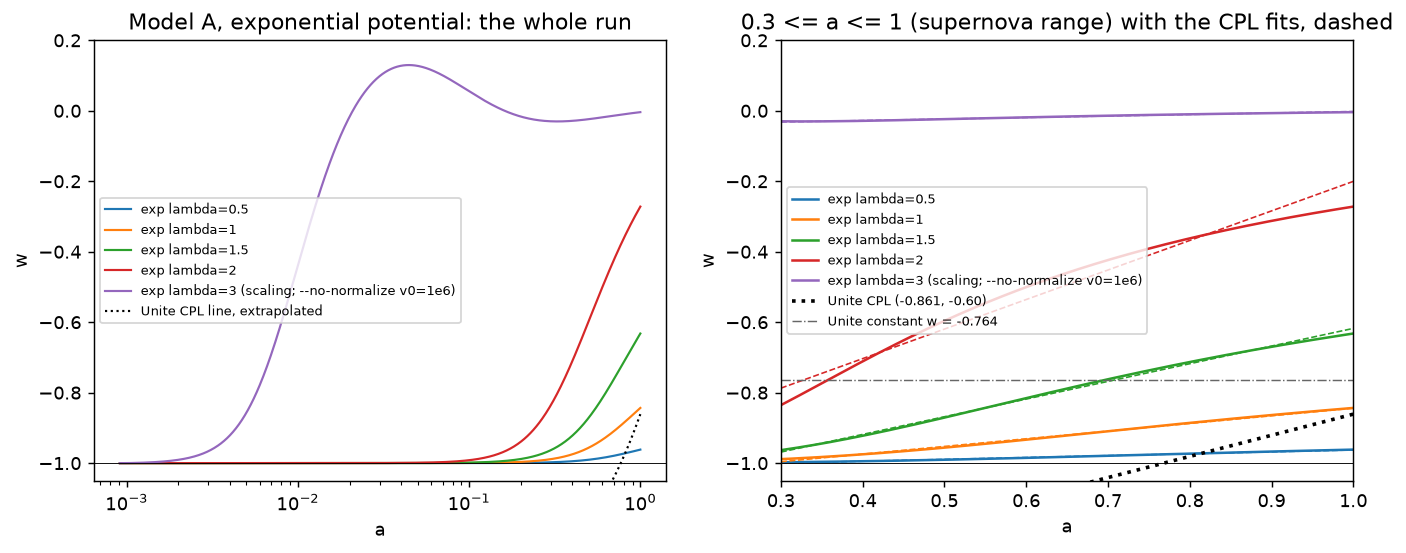
\includegraphics[width=\textwidth]{nb01_w_of_a_exp.png}
\caption{Model A, exponential potential. Left: $w(a)$ over the whole run, with Unite's CPL line
extrapolated (dotted). Right: the supernova range $0.3\le a\le1$ with each run's CPL fit (dashed),
Unite's line (dotted) and the constant-$w$ fit $-0.764$ (dash-dotted). The $\lambda=3$ run is the
scaling solution with $V_0=10^6$ set by hand.}
\label{fig:expw}
\end{figure}

\paragraph{The other potentials.} The inverse power ($\alpha=1$) does not join its tracker
($w=-2/3$ in the matter era) from a frozen start: starting at $N_0=-7$ or at $N_0=-25$ gives the
same history to $3.0\times10^{-8}$ in $w$, because Hubble friction in the radiation era holds the
field frozen ($w(N=-4)=-0.99975$, $w(N=-2)=-0.92110$); it thaws late, overshoots and turns down,
$w(1)=-0.7532$, with fit $(-0.7365,+0.0625)$, class \emph{mixed}. The PNGB potentials thaw mildly
($f=1$: $(-0.9888,-0.0165)$; $f=0.5$ from $\phi_i=0.3$: $(-0.8841,-0.1817)$), the hilltop with
$\mu=3$ is almost frozen ($(-0.9993,-0.0010)$), and the control is $w=-1$ to machine precision
(Figure~\ref{fig:otherw}).

\begin{figure}[htbp]
\centering
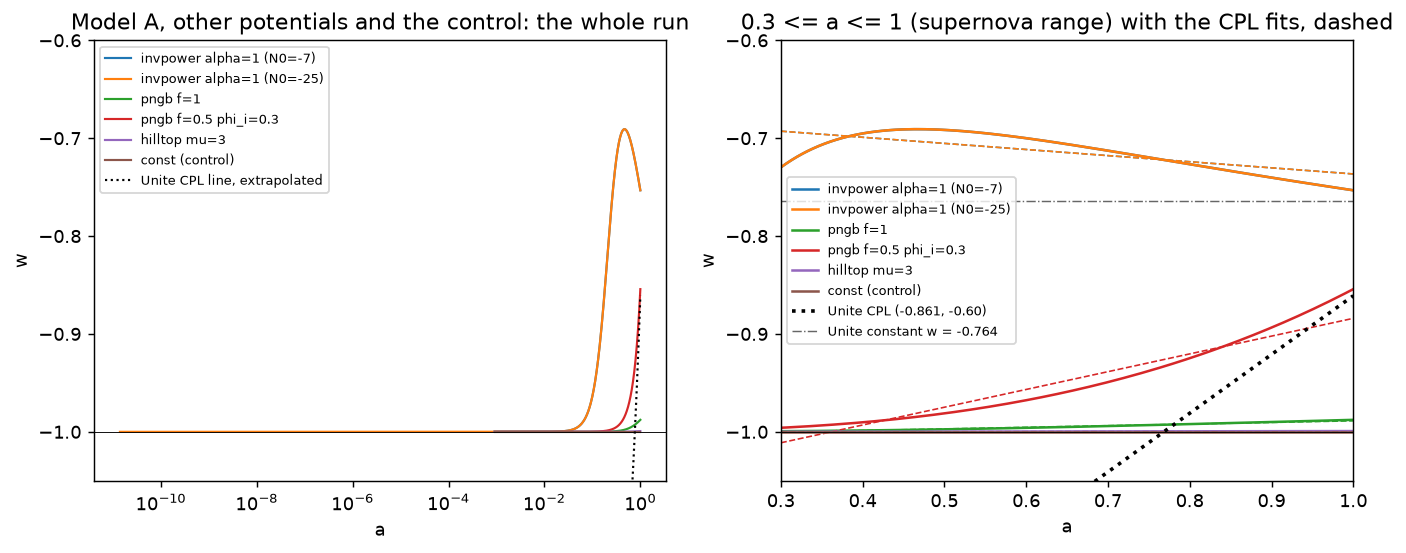
\includegraphics[width=\textwidth]{nb01_w_of_a_other.png}
\caption{Model A, the inverse-power (two starts, indistinguishable), PNGB, hilltop and constant
potentials; panels as in Figure~\ref{fig:expw}.}
\label{fig:otherw}
\end{figure}

\paragraph{Model A$'$.} As a test field on the Unite CPL background, $\lambda=1$ gives
$w(1)=-0.8391$ and fit $(-0.8371,-0.2257)$, essentially the self-consistent result. $\lambda=2$
cannot carry $\Omega_{DE}=0.70$ ($\rho_\phi(10^6V)=1.025<2.100$): a test field with $\lambda^2>3$
scales with the background; run by hand with $V_0=10$ it carries $\Omega=0.4984$ today, with
$w(1)=-0.2980$ (Figure~\ref{fig:cplw}).

\begin{figure}[htbp]
\centering
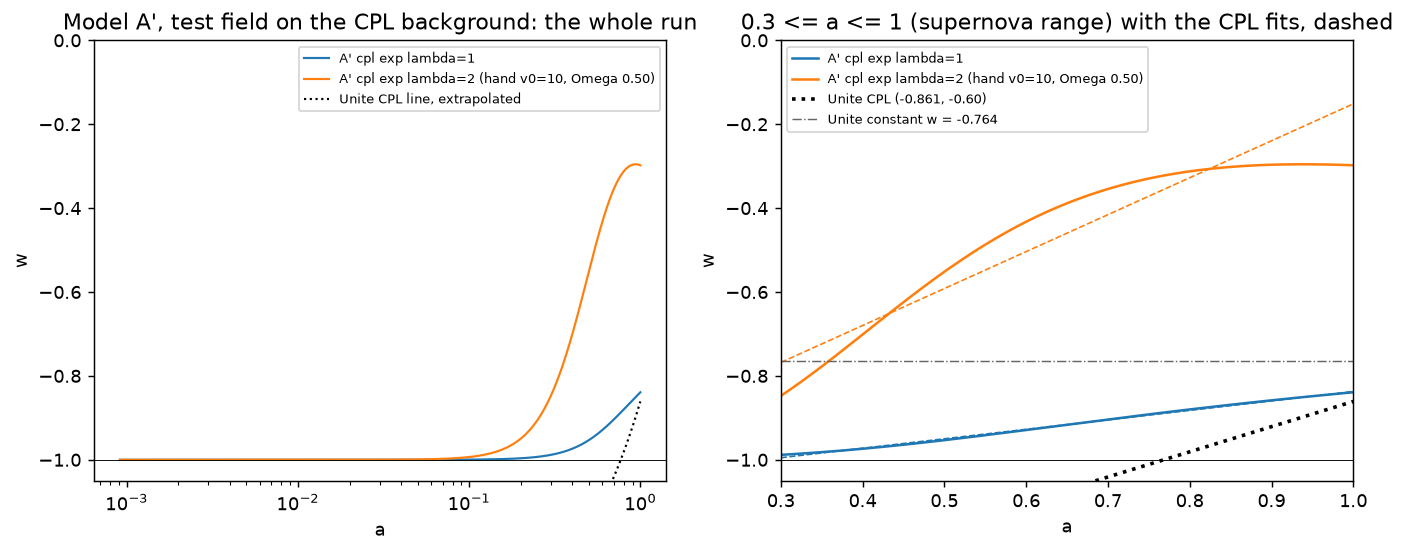
\includegraphics[width=\textwidth]{nb01_w_of_a_cpl.png}
\caption{Model A$'$: the exponential \fableScalar{} as a test field on the Unite CPL background
($\lambda=1$ normalised; $\lambda=2$ with $V_0=10$ by hand, $\Omega=0.50$ today).}
\label{fig:cplw}
\end{figure}

\paragraph{Thawing, and where the exponential lands in the CPL plane.} In the Caldwell--Linder
plane (Figure~\ref{fig:cl1}, left) every exponential, PNGB and hilltop run stays above
$w'=\dd w/\dd N=0$ over the fit range: thawing; the inverse-power runs cross the axis: mixed. A
scan $\lambda=0.5,0.6,\dots,2.0$ (Figure~\ref{fig:cl1}, right; \file{results/nb01_lambda_scan.csv})
moves the fit monotonically from $(-0.9627,-0.0532)$ to $(-0.2004,-0.8384)$. The distance from
Unite's point is smallest at $\lambda=1.4$, $(w_0,w_a)=(-0.6740,-0.4349)$, distance $0.2495$; the
fitted $w_a$ reaches $-0.60$ at $\lambda=1.638$, where $w_0=-0.5274$. Table~\ref{tab:fitsA} lists
the fits.

\begin{figure}[htbp]
\centering
\begin{subfigure}[t]{0.52\textwidth}
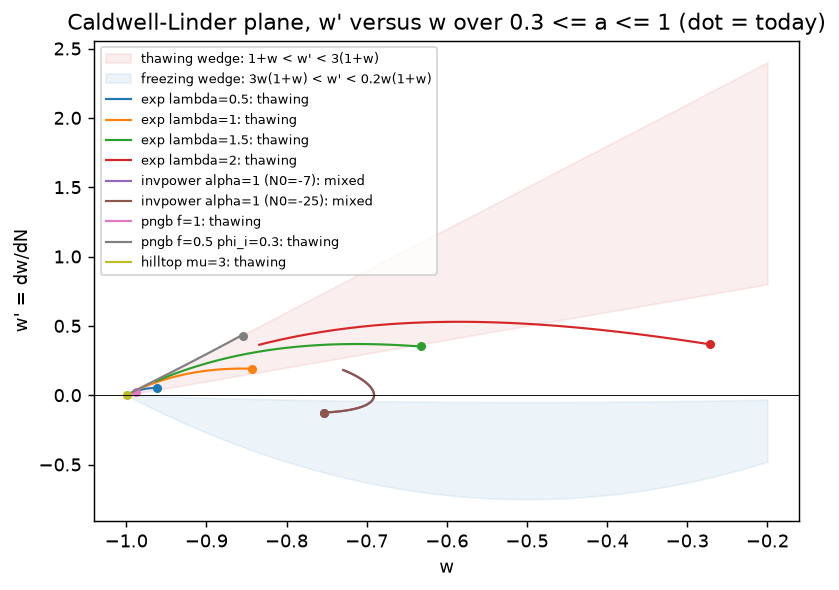
\includegraphics[width=\linewidth]{nb01_caldwell_linder.png}
\caption{The Caldwell--Linder plane $w'$ versus $w$, $0.3\le a\le1$; dots mark today.}
\end{subfigure}\hfill
\begin{subfigure}[t]{0.46\textwidth}
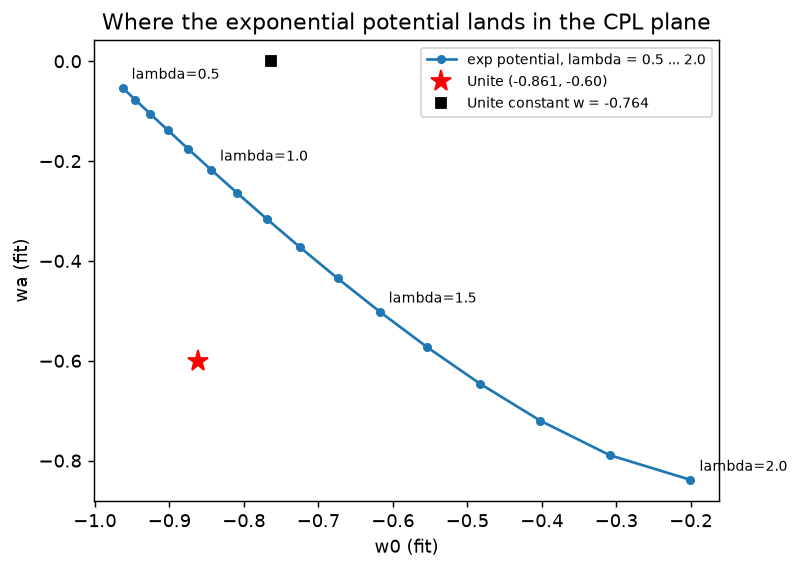
\includegraphics[width=\linewidth]{nb01_lambda_scan.png}
\caption{The fitted $(w_0,w_a)$ of the exponential potential for $\lambda=0.5\dots2.0$.}
\end{subfigure}
\caption{Model A: classification and the path of the CPL fit.}
\label{fig:cl1}
\end{figure}

\begin{table}[htbp]
\centering\small
\caption{CPL fits over $0.3\le a\le1$ of Models A and A$'$ (\texttt{results/nb01\_cpl\_fits.csv}).
$\min w=-1$ for every run; ``dist'' is the distance of $(w_0,w_a)$ from Unite's point.}
\label{tab:fitsA}
\begin{tabular}{@{}l r r r r r l r@{}}
\toprule
run & $w_0$ & $w_a$ & $w_0+w_a$ & $w(0.3)$ & $w(1)$ & class & dist \\
\midrule
\texttt{exp} $\lambda=0.5$ & $-0.9627$ & $-0.0532$ & $-1.0159$ & $-0.9976$ & $-0.9616$ & thawing & 0.556 \\
\texttt{exp} $\lambda=1$ & $-0.8440$ & $-0.2172$ & $-1.0612$ & $-0.9887$ & $-0.8434$ & thawing & 0.383 \\
\texttt{exp} $\lambda=1.5$ & $-0.6176$ & $-0.5015$ & $-1.1191$ & $-0.9632$ & $-0.6322$ & thawing & 0.263 \\
\texttt{exp} $\lambda=2$ & $-0.2004$ & $-0.8384$ & $-1.0388$ & $-0.8355$ & $-0.2720$ & thawing & 0.702 \\
\texttt{exp} $\lambda=3$ (scaling, $\Omega=0.34$) & $-0.0020$ & $-0.0427$ & $-0.0448$ & $-0.0299$ & $-0.0039$ & mixed & 1.024 \\
\texttt{invpower} $\alpha=1$ ($N_0=-7$) & $-0.7365$ & $+0.0625$ & $-0.6741$ & $-0.7298$ & $-0.7532$ & mixed & 0.674 \\
\texttt{pngb} $f=1$ & $-0.9888$ & $-0.0165$ & $-1.0053$ & $-0.9994$ & $-0.9878$ & thawing & 0.597 \\
\texttt{pngb} $f=0.5$, $\phi_i=0.3$ & $-0.8841$ & $-0.1817$ & $-1.0657$ & $-0.9959$ & $-0.8542$ & thawing & 0.419 \\
\texttt{hilltop} $\mu=3$ & $-0.9993$ & $-0.0010$ & $-1.0003$ & $-1.0000$ & $-0.9992$ & thawing & 0.615 \\
\texttt{const} (control) & $-1.0000$ & $0.0000$ & $-1.0000$ & $-1.0000$ & $-1.0000$ & constant & 0.616 \\
A$'$ \texttt{exp} $\lambda=1$ & $-0.8371$ & $-0.2257$ & $-1.0628$ & $-0.9883$ & $-0.8391$ & thawing & 0.375 \\
A$'$ \texttt{exp} $\lambda=2$ ($\Omega=0.50$) & $-0.1515$ & $-0.8806$ & $-1.0321$ & $-0.8476$ & $-0.2980$ & mixed & 0.763 \\
\midrule
Unite CPL & $-0.861$ & $-0.60$ & $-1.461$ & $-1.281$ & $-0.861$ & & 0 \\
Unite constant $w$ & $-0.764$ & $0$ & $-0.764$ & $-0.764$ & $-0.764$ & & 0.608 \\
\bottomrule
\end{tabular}
\end{table}

\FloatBarrier
\subsection{\fable{} in the reference model (Model B)}

\paragraph{Dust and $\Lambda$.} The \texttt{mass} spinor has $w=0$ at every point and
$\rho_\Psi a^3$ constant to $5.3\times10^{-8}$ (CVODE's error on $s$). \texttt{lambda-mass} with
$V_0=0.7$, $m=0.3$ before normalisation ($1.469824$ and $0.629924$ after) splits into
$\Omega_\Lambda=V(0)/3=0.489941$, a bare constant in the action, and spinor dust
$\Omega_{\mathrm{dust}}=ms_0/3=0.209975$; $w(1)=-V_0/(V_0+ms_0)=-0.700000$. It is $\Lambda$CDM with
the dust supplied by the spinor. The \texttt{power} potentials with $m=\lambda$ are dust early and
tend to $n-1$ late: $w(1)=-0.38200$, $-0.25000$, $-0.05000$ for $n=0.236$, $0.5$, $0.9$
($w(a=0.1)=-0.00388$, $-0.01533$, $-0.03339$); run into the future to $N=+6$ the $n=0.236$ case
reaches $w=-0.76399919$, Unite's constant value to $8.1\times10^{-7}$ (Figures~\ref{fig:pot},
\ref{fig:dust}).

\begin{figure}[htbp]
\centering
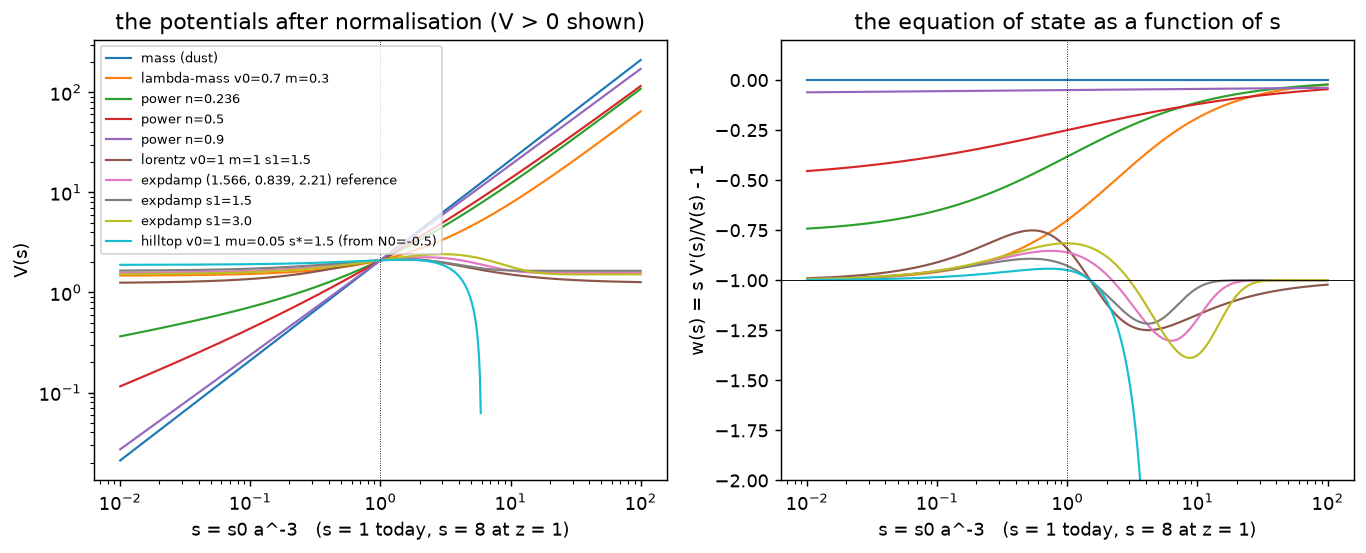
\includegraphics[width=\textwidth]{nb02_potentials.png}
\caption{The potentials of \fable{} after normalisation (left, $V>0$ shown) and $w(s)=sV'/V-1$
(right), against $s=s_0a^{-3}$; $s=1$ today, $s=8$ at $z=1$. Where $V'$ changes sign $w$ crosses
$-1$.}
\label{fig:pot}
\end{figure}

\begin{figure}[htbp]
\centering
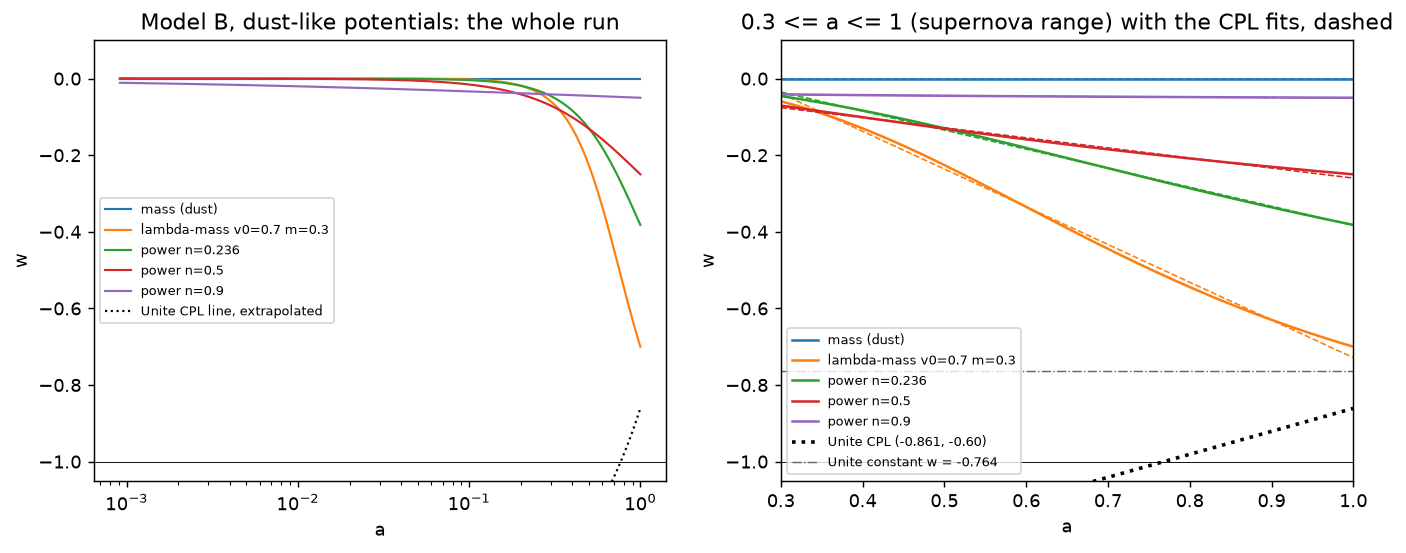
\includegraphics[width=\textwidth]{nb02_w_of_a_dust.png}
\caption{Model B, the dust-like potentials: \texttt{mass}, \texttt{lambda-mass} and
\texttt{power}; panels as in Figure~\ref{fig:expw}.}
\label{fig:dust}
\end{figure}

\paragraph{Crossing the phantom divide.} \texttt{lorentz}, \texttt{expdamp} (three values of
$s_1$) and \texttt{hilltop} all cross $w=-1$ exactly once, at the analytic scale factor
(Table~\ref{tab:crossings}, Figure~\ref{fig:phantom}). The reference \texttt{expdamp}
$(1.566,0.839,2.21)$ has $w(1)=-0.86085$, crosses $-1$ at $a_c=0.7677$ ($z=0.30$), reaches
$w=-1.30210$ at $a=0.5434$ ($z=0.840$) and tends to $-1$ from below as $a\to0$; $V$ never falls
below $V_0=1.566$, so $\rho_\Psi>0$ throughout. The \texttt{hilltop} is refused from the default
start ($V(s)=-1.8\times10^{17}$ at $s=1.3188\times10^{9}$) and is run only inside its window
$s<s_*+\sqrt{V_0/\mu}=5.9721$ ($a>0.5512$), from $N_0=-0.5$.

\begin{figure}[htbp]
\centering
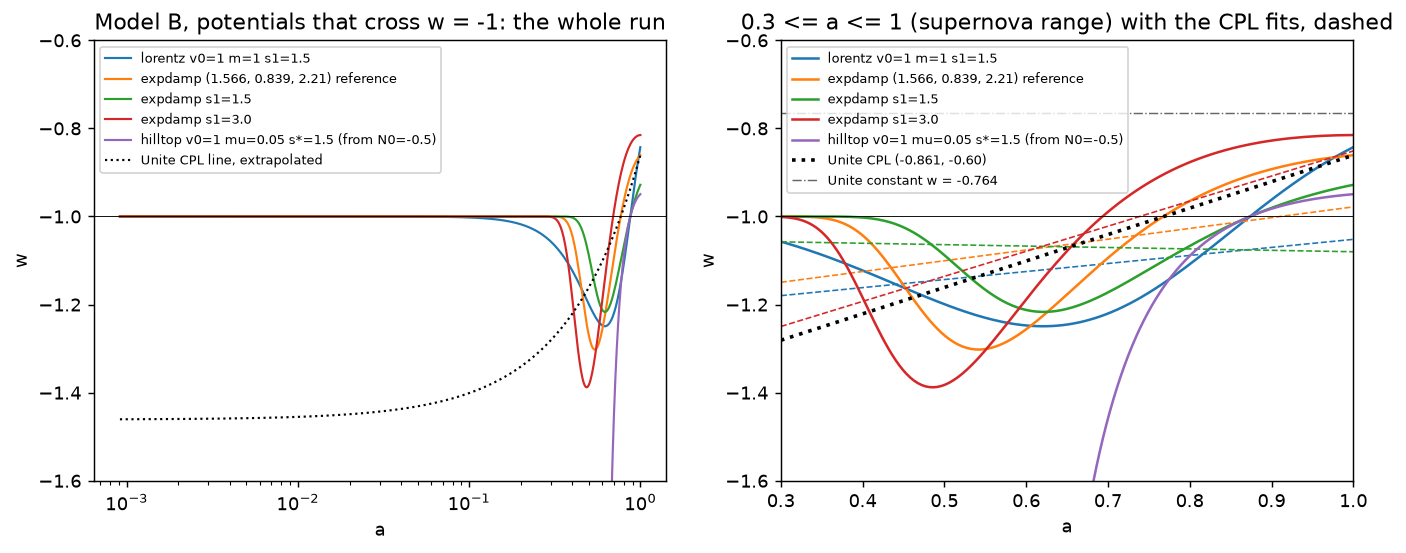
\includegraphics[width=\textwidth]{nb02_w_of_a_phantom.png}
\caption{Model B, the potentials that cross $w=-1$: \texttt{lorentz}, \texttt{expdamp}
(reference, $s_1=1.5$, $s_1=3.0$) and \texttt{hilltop} (from $N_0=-0.5$); panels as in
Figure~\ref{fig:expw}.}
\label{fig:phantom}
\end{figure}

\begin{table}[htbp]
\centering\small
\caption{Crossings of $w=-1$ in Model B, numerical (local degree-6 polynomial and root bracket
on the 701-point grid) against the analytic $a_c=(s_1/s_0)^{-1/3}$
(\texttt{results/nb02\_crossings.csv}).}
\label{tab:crossings}
\begin{tabular}{@{}l l l l l@{}}
\toprule
run & $a_c$ numerical & $a_c$ analytic & $|\Delta|$ & $\min V$ \\
\midrule
\texttt{lorentz} $V_0=m=1$, $s_1=1.5$ & 0.8735804797 & 0.8735804647 & $1.50\times10^{-8}$ & 1.2408 \\
\texttt{expdamp} $(1.566,0.839,2.21)$ & 0.7677195193 & 0.7677195065 & $1.29\times10^{-8}$ & 1.5660 \\
\texttt{expdamp} $s_1=1.5$ & 0.8735804797 & 0.8735804647 & $1.50\times10^{-8}$ & 1.6468 \\
\texttt{expdamp} $s_1=3.0$ & 0.6933612858 & 0.6933612744 & $1.15\times10^{-8}$ & 1.5173 \\
\texttt{hilltop} $s_*=1.5$ (from $N_0=-0.5$) & 0.8735804648 & 0.8735804647 & $4.00\times10^{-11}$ & 1.1811 \\
\bottomrule
\end{tabular}
\end{table}

\begin{table}[htbp]
\centering\small
\caption{CPL fits over $0.3\le a\le1$ of Model B (\texttt{results/nb02\_cpl\_fits.csv}). The hilltop
run starts at $a=0.61$, so its fit covers $0.61\le a\le1$ and its $w(0.3)$ is undefined.}
\label{tab:fitsB}
\setlength{\tabcolsep}{4pt}
\begin{tabular}{@{}l r r r r r r l r@{}}
\toprule
run & $w_0$ & $w_a$ & $w_0+w_a$ & $w(0.3)$ & $w(1)$ & $\min w$ & class & dist \\
\midrule
\texttt{mass} & $0.0000$ & $0.0000$ & $0.0000$ & $0.0000$ & $0.0000$ & $0.0000$ & constant & 1.049 \\
\texttt{lambda-mass} & $-0.7286$ & $+0.9850$ & $+0.2564$ & $-0.0593$ & $-0.7000$ & $-0.7000$ & freezing & 1.591 \\
\texttt{power} $n=0.236$ & $-0.3830$ & $+0.4971$ & $+0.1141$ & $-0.0455$ & $-0.3820$ & $-0.3820$ & freezing & 1.197 \\
\texttt{power} $n=0.5$ & $-0.2598$ & $+0.2630$ & $+0.0032$ & $-0.0706$ & $-0.2500$ & $-0.2500$ & freezing & 1.052 \\
\texttt{power} $n=0.9$ & $-0.0508$ & $+0.0128$ & $-0.0381$ & $-0.0411$ & $-0.0500$ & $-0.0500$ & freezing & 1.016 \\
\texttt{lorentz} & $-1.0519$ & $-0.1826$ & $-1.2346$ & $-1.0570$ & $-0.8427$ & $-1.2492$ & mixed & 0.459 \\
\texttt{expdamp} reference & $-0.9782$ & $-0.2445$ & $-1.2227$ & $-1.0000$ & $-0.8608$ & $-1.3021$ & mixed & 0.374 \\
\texttt{expdamp} $s_1=1.5$ & $-1.0801$ & $+0.0322$ & $-1.0479$ & $-1.0000$ & $-0.9281$ & $-1.2166$ & mixed & 0.669 \\
\texttt{expdamp} $s_1=3.0$ & $-0.8513$ & $-0.5692$ & $-1.4205$ & $-1.0010$ & $-0.8151$ & $-1.3878$ & mixed & 0.032 \\
\texttt{hilltop} (from $a=0.61$) & $-0.5265$ & $-4.0285$ & $-4.5550$ & --- & $-0.9494$ & $-3.4057$ & thawing & 3.445 \\
\bottomrule
\end{tabular}
\end{table}

The straight line is a poor description of a $w(a)$ that dips to $-1.3$ and comes back
(Table~\ref{tab:fitsB}): the reference \texttt{expdamp} fits $(-0.9782,-0.2445)$ although its
$w(1)$ is $-0.861$. In the Caldwell--Linder plane (Figure~\ref{fig:cl2}) the phantom runs sit at
$w<-1$ in the past and rise through the divide towards today, so their $\dd w/\dd N$ changes sign
over the fit range: mixed. The dust-like runs are freezing.

\begin{figure}[htbp]
\centering
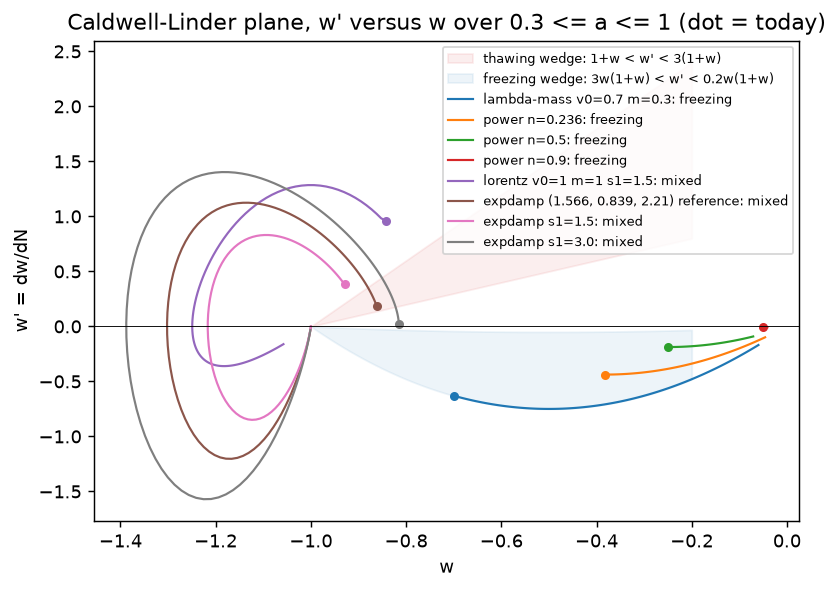
\includegraphics[width=0.62\textwidth]{nb02_caldwell_linder.png}
\caption{Model B in the Caldwell--Linder plane, $0.3\le a\le1$; dots mark today.}
\label{fig:cl2}
\end{figure}

\FloatBarrier
\subsection{\fableScalar{} on the pre-universe (Models C and D)}

\paragraph{Model C.} The quadratic potential ($m=1$, $\phi_i=1$, to $x^4=100$, 2001 outputs)
reproduces the exact solution $\phi=\cos x^4$ to $1.67\times10^{-9}$ and $w=-\cos 2x^4$ to
$2.05\times10^{-9}$; $w$ swings between $-1$ and $+1$ while $\rho=\tfrac12$ is conserved to
$3.27\times10^{-9}$, and the running average is $w_{\mathrm{avg}}(100)=+0.004363$
(Figure~\ref{fig:modelC}). The quartic potential ($\lambda=1$) averages to
$w_{\mathrm{avg}}(100)=0.334909$, within $1.6\times10^{-3}$ of the virial value $1/3$: the
oscillating field averages to radiation; $\rho$ is conserved to $1.58\times10^{-8}$
(Figure~\ref{fig:modelC4}). The residuals of the averages are the last incomplete period divided
by the length of the run.

\begin{figure}[htbp]
\centering
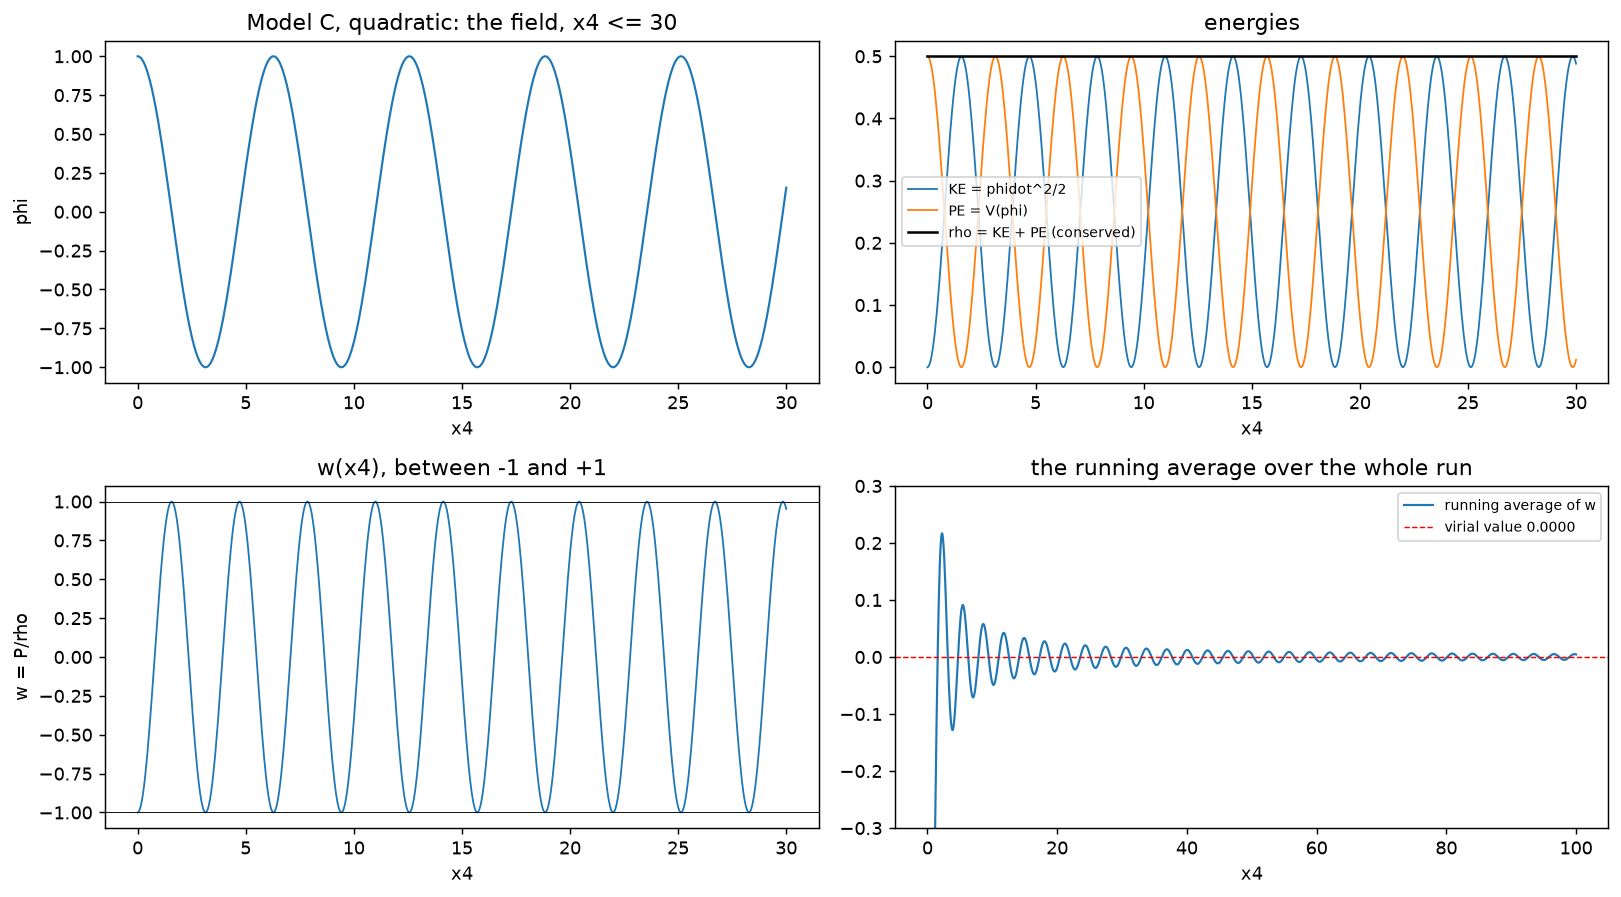
\includegraphics[width=\textwidth]{nb03_modelC_quadratic.png}
\caption{Model C, quadratic potential, on the pre-universe: no Hubble friction. The field, the
exchange of kinetic and potential energy at constant $\rho$, $w(x^4)$ between $-1$ and $+1$, and
its running average settling on the virial value $0$.}
\label{fig:modelC}
\end{figure}

\begin{figure}[htbp]
\centering
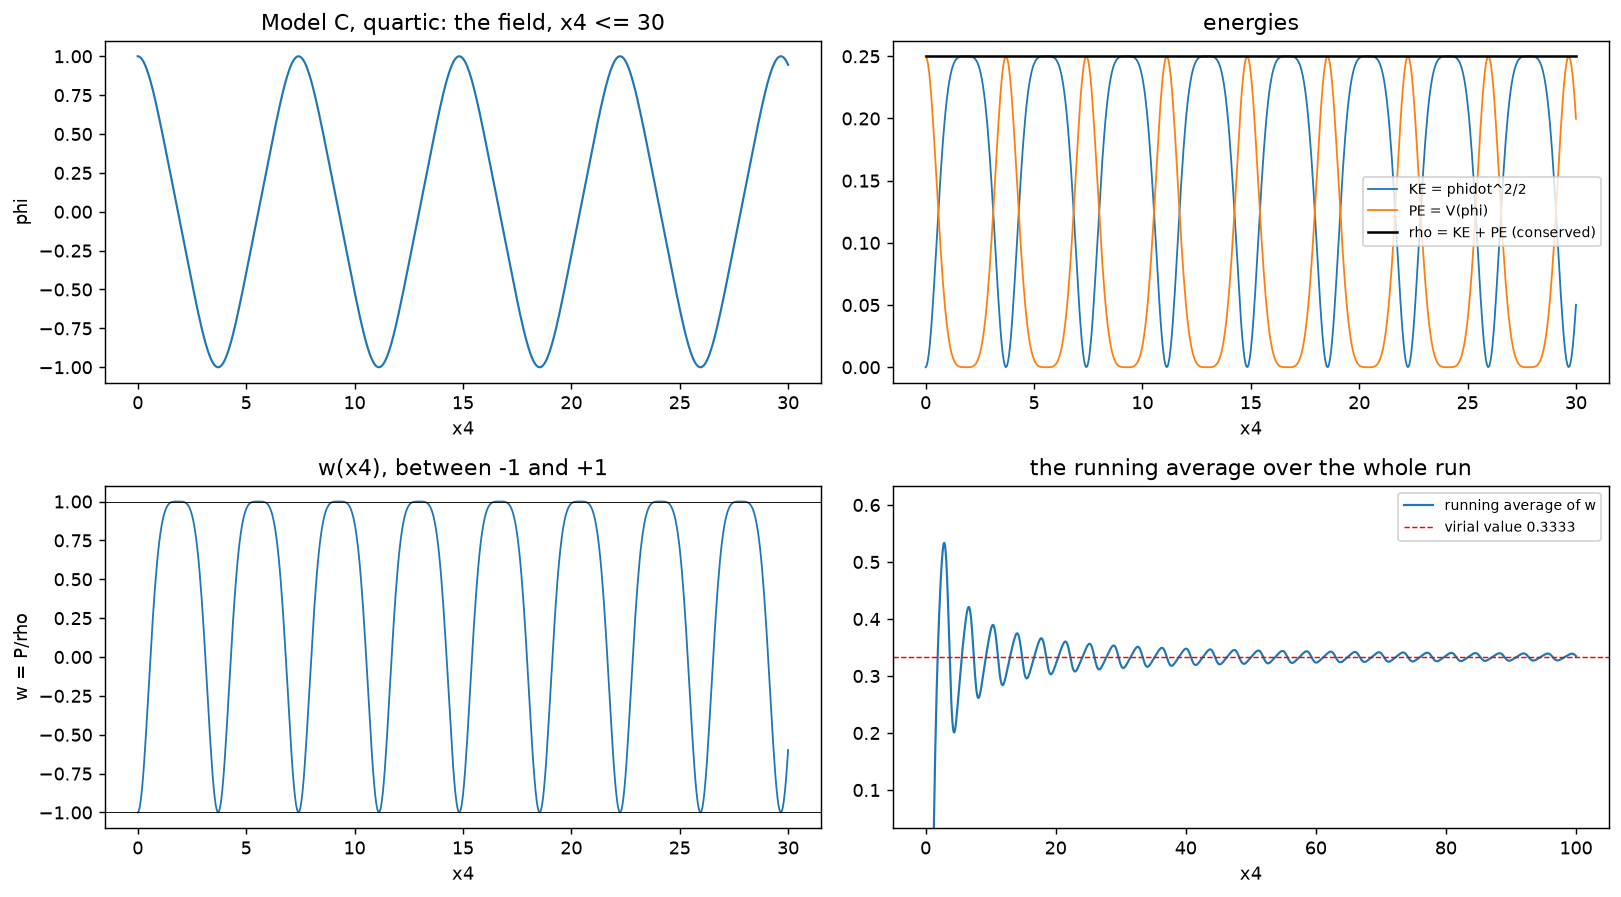
\includegraphics[width=\textwidth]{nb03_modelC_quartic.png}
\caption{Model C, quartic potential: the running average of $w$ settles on the virial value
$1/3$.}
\label{fig:modelC4}
\end{figure}

\paragraph{Model D: the sloshing mechanism.} The quadratic potential on 61 grid points in
$x^0\in[0.05,0.22]$, from a profile at rest, to $x^4=30$ (Figures~\ref{fig:modelD05},
\ref{fig:modelD5}). Because the flux coefficient $\sec\cot^2$ is large near $x^0=0.05$
($\cot^2 0.3=10.4$), even a 5\,\% ripple ($\varepsilon=0.05$) stores $28.5\,\%$ of $E_h$ in $G_0$ at
the start. The gradient store exchanges energy with the $x^4$ motion: for $\varepsilon=0.05$ the
$G_0$ fraction ranges over $[0.0288,0.2847]$ and $w_{\mathrm{sheet}}$ over $[-1,+0.9412]$; for
$\varepsilon=0.5$, $97.8\,\%$ of $E_h$ starts in $G_0$, the fraction falls to $9.88\,\%$ and comes
back, and $w_{\mathrm{sheet}}$ ranges over $[-1,+0.8022]$. Because the quadratic problem is linear,
the virial theorem holds for the whole sheet, $\langle\mathrm{KE}\rangle=\langle\mathrm{PE}\rangle
+\langle G_0\rangle$: the time-averaged kinetic fractions are $0.5017$ and $0.4997$ and the running
averages of $w_{\mathrm{sheet}}$ at $x^4=30$ are $+0.0038$ and $+0.0007$. The gradient store changes
the history of $w$, not its average; only a massless profile stays at $w=-1$. $E_h$ is conserved to
$4.48\times10^{-9}$ and $9.05\times10^{-9}$.

\begin{figure}[htbp]
\centering
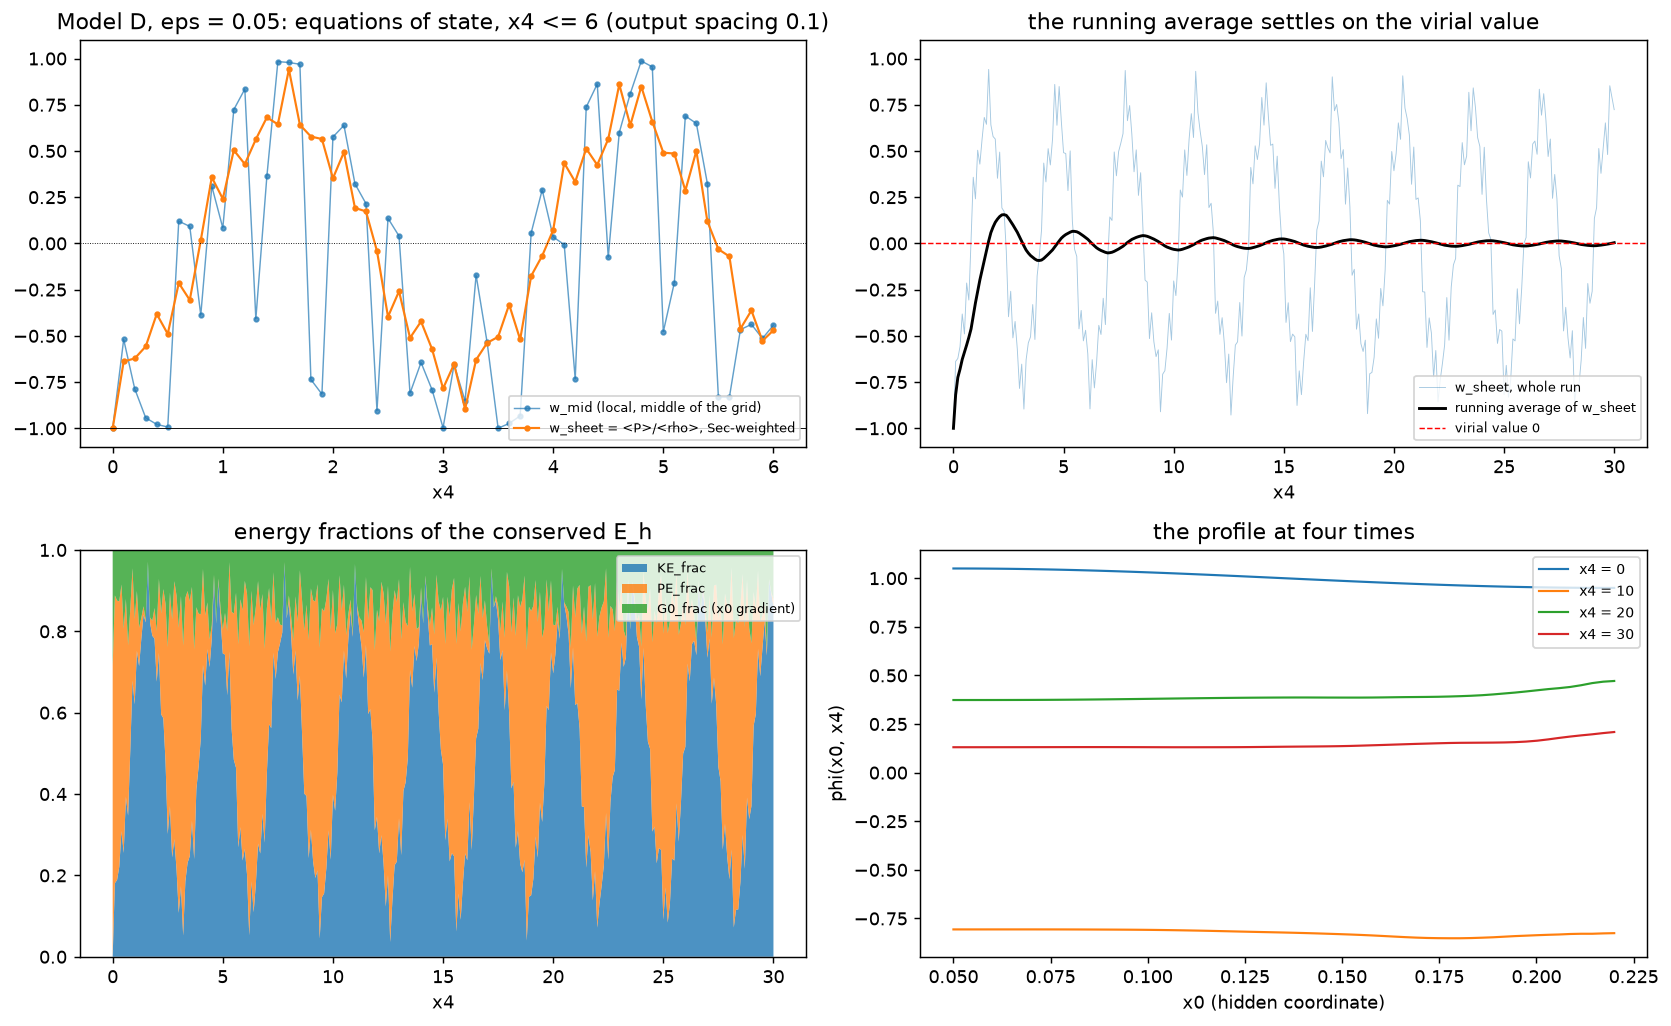
\includegraphics[width=\textwidth]{nb03_modelD_eps0.05.png}
\caption{Model D, $\varepsilon=0.05$: the local $w_{\mathrm{mid}}$ and the $\sec$-weighted
$w_{\mathrm{sheet}}=\langle P\rangle/\langle\rho\rangle$ over $x^4\le6$ (dots are the outputs, spacing
0.1); the running average of $w_{\mathrm{sheet}}$; the energy fractions of the conserved $E_h$;
the profile $\phi(x^0)$ at four times.}
\label{fig:modelD05}
\end{figure}

\begin{figure}[htbp]
\centering
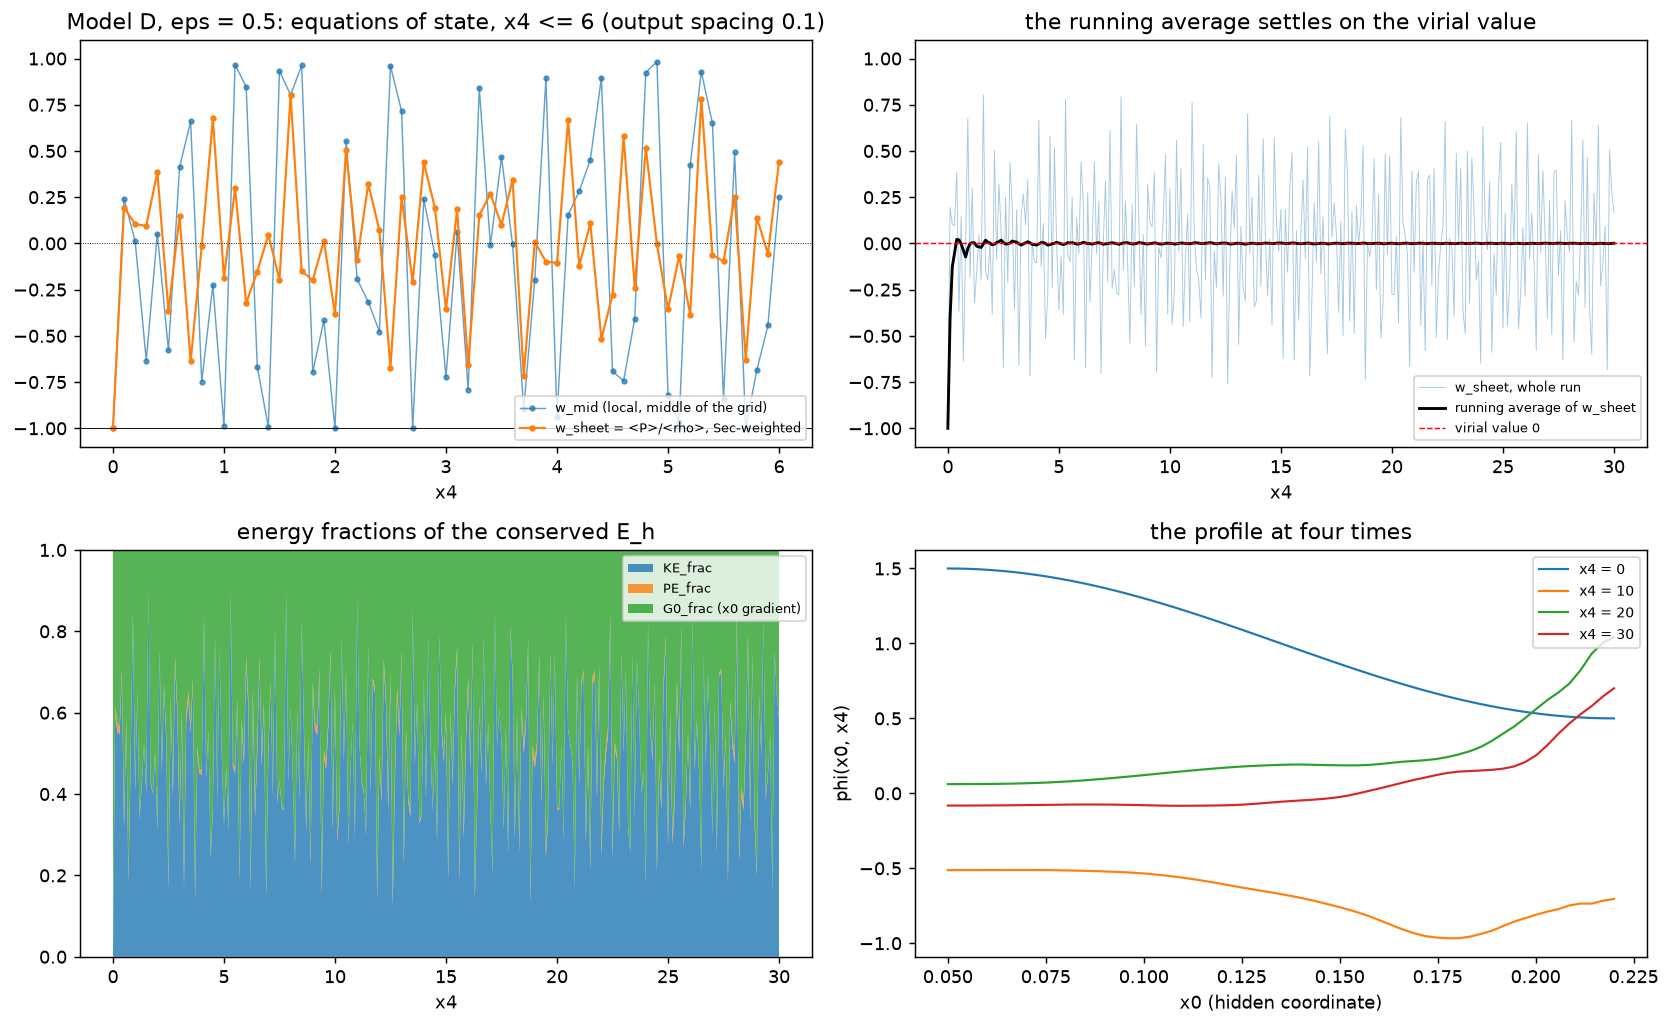
\includegraphics[width=\textwidth]{nb03_modelD_eps0.5.png}
\caption{Model D, $\varepsilon=0.5$; panels as in Figure~\ref{fig:modelD05}. Most of the energy
starts in the $x^0$ gradient, a $w=-1$ store on the observed sheet, and sloshes into the $x^4$
motion and back.}
\label{fig:modelD5}
\end{figure}

\paragraph{Model E.} For \fable{} on the pre-universe nothing needs integrating: $\partial_4 s=0$
exactly (F3), so $V$, $\rho_\Psi$ and $w_\Psi$ are constant along the observer's time. The $a^{-3}$
dilution of Model B is the reference model's Hubble term, which the pre-universe does not have.

\FloatBarrier
\subsection{The synthesis}\label{sec:synthesis}

Figure~\ref{fig:all} shows the best cases of both fields against Unite's line.
Figure~\ref{fig:omega} shows the density fractions: at the start radiation is $\Omega_r=0.2349$;
the field overtakes matter at $a=0.7376$ ($z=0.356$) for the reference \texttt{expdamp} spinor and
at $a=0.7239$ ($z=0.381$) for the $\lambda=1$ scalar. Figure~\ref{fig:qdec} shows the
deceleration parameter: acceleration begins ($q_{\mathrm{dec}}=0$) at $a=0.5475$ ($z=0.827$) for
the reference \texttt{expdamp}, $a=0.5840$ ($z=0.712$) for the $\lambda=1$ scalar and $a=0.8045$
($z=0.243$) for \texttt{lambda-mass}, and never for the \texttt{mass} spinor
($q_{\mathrm{dec}}(1)=+0.5000$). Today $q_{\mathrm{dec}}=-0.4037$, $-0.3854$, $-0.2349$ for these three,
$-0.3557$ for \texttt{expdamp} $s_1=3.0$, $-0.1637$ for \texttt{exp} $\lambda=1.5$ and $+0.0990$ for
\texttt{power} $n=0.236$ with $m=\lambda$, which does not accelerate today. The age today is
$t(1)=0.9472/H_0$ for the $\lambda=1$ scalar, $0.9643/H_0$ for the reference \texttt{expdamp},
$0.9637/H_0$ for the \texttt{const} control and $0.6666/H_0$ for the \texttt{mass} spinor (all dust:
the Einstein--de Sitter $2/3$).

\begin{figure}[htbp]
\centering
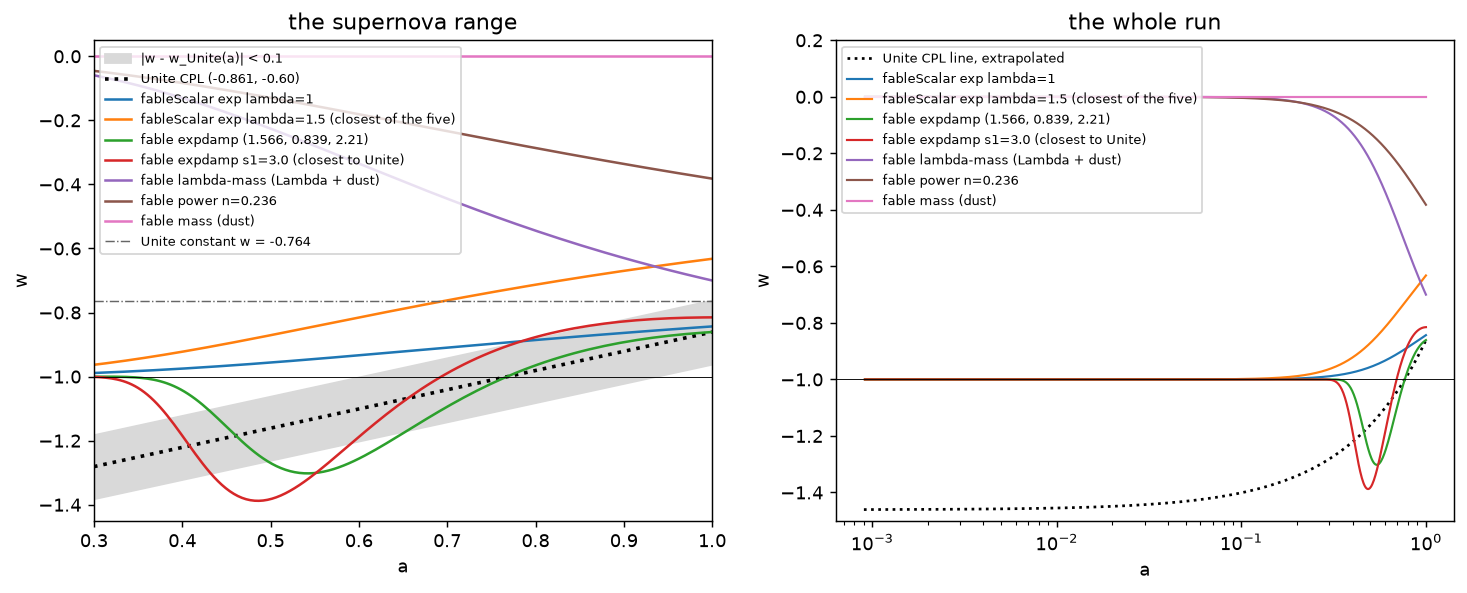
\includegraphics[width=\textwidth]{nb04_w_of_a_all.png}
\caption{The best cases of both fields. Left: the supernova range with Unite's CPL line and the
band $|w-w_{\mathrm{Unite}}(a)|<0.1$. Right: the whole run with the CPL line extrapolated.}
\label{fig:all}
\end{figure}

\begin{figure}[htbp]
\centering
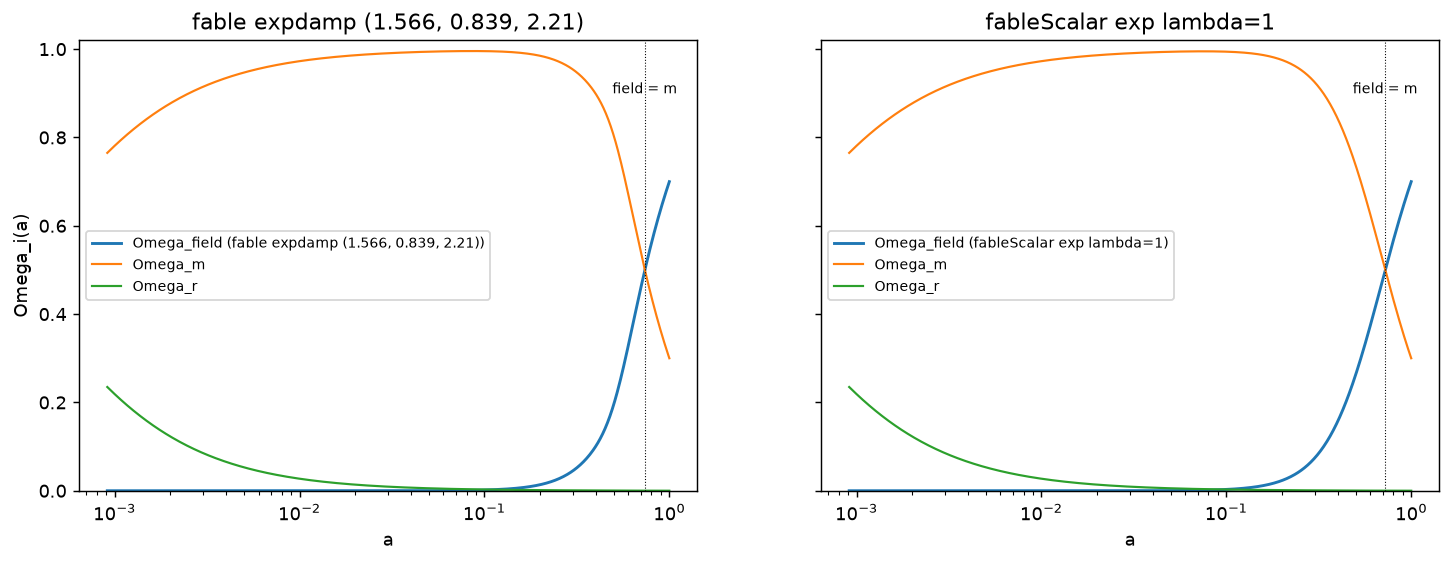
\includegraphics[width=\textwidth]{nb04_omega_history.png}
\caption{Density fractions $\Omega_{\mathrm{field}}$, $\Omega_m$, $\Omega_r$ for the reference
\texttt{expdamp} spinor (left) and the $\lambda=1$ exponential scalar (right); the dotted line
marks where the field overtakes matter.}
\label{fig:omega}
\end{figure}

\begin{figure}[htbp]
\centering
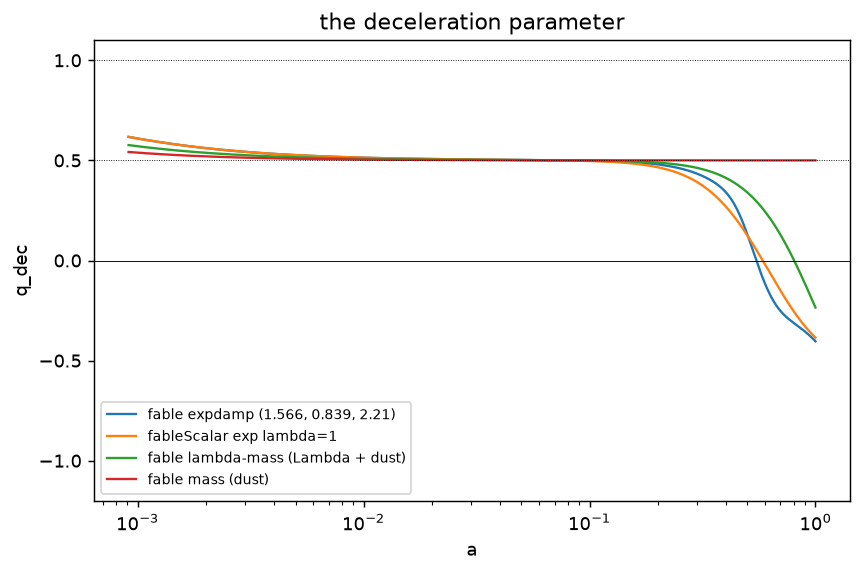
\includegraphics[width=0.62\textwidth]{nb04_deceleration.png}
\caption{The deceleration parameter $q_{\mathrm{dec}}=-1-(\dd H/\dd N)/H$.}
\label{fig:qdec}
\end{figure}

\FloatBarrier
% =====================================================================================
\section{Comparison with the Supernovae Unite fits}\label{sec:unite}

\begin{table}[htbp]
\centering\small
\caption{The runs closest to Unite's $(w_0,w_a)=(-0.861,-0.60)$, sorted by distance, with the
constant-$w$ reference. All fits over $0.3\le a\le1$.}
\label{tab:unite}
\setlength{\tabcolsep}{4pt}
\begin{tabular}{@{}l l r r r r r r@{}}
\toprule
run & model & $w_0$ & $w_a$ & $w_0+w_a$ & $w(1)$ & $\min w$ & dist \\
\midrule
Unite CPL & & $-0.861$ & $-0.60$ & $-1.461$ & $-0.861$ & & 0 \\
\texttt{expdamp} $s_1=3.0$ & B & $-0.8513$ & $-0.5692$ & $-1.4205$ & $-0.8151$ & $-1.3878$ & 0.032 \\
\texttt{exp} $\lambda=1.4$ (scan) & A & $-0.6740$ & $-0.4349$ & $-1.1089$ & $-0.6832$ & $-1.0000$ & 0.250 \\
\texttt{exp} $\lambda=1.5$ & A & $-0.6176$ & $-0.5015$ & $-1.1191$ & $-0.6322$ & $-1.0000$ & 0.263 \\
\texttt{expdamp} reference & B & $-0.9782$ & $-0.2445$ & $-1.2227$ & $-0.8608$ & $-1.3021$ & 0.374 \\
\texttt{exp} $\lambda=1$ on the CPL background & A$'$ & $-0.8371$ & $-0.2257$ & $-1.0628$ & $-0.8391$ & $-1.0000$ & 0.375 \\
\texttt{exp} $\lambda=1$ & A & $-0.8440$ & $-0.2172$ & $-1.0612$ & $-0.8434$ & $-1.0000$ & 0.383 \\
\texttt{lorentz} & B & $-1.0519$ & $-0.1826$ & $-1.2346$ & $-0.8427$ & $-1.2492$ & 0.459 \\
\midrule
Unite constant $w$ & & $-0.764$ & $0$ & $-0.764$ & $-0.764$ & & 0.608 \\
\texttt{power} $n=0.236$, late times & B & \multicolumn{6}{l}{$w\to n-1=-0.764$; $w(N=6)=-0.76399919$} \\
\bottomrule
\end{tabular}
\end{table}

Table~\ref{tab:unite} collects the comparison. Three conclusions follow.

\emph{A thawing \fableScalar{} gives Unite's sign pattern but not the pair.} Every exponential
run of the scan $\lambda=0.5,\dots,2.0$ has $w_0>-1$ and $w_a<0$, and its CPL extrapolation
$w_0+w_a$ lies below $-1$ (between $-1.016$ and $-1.129$; $-1.06$ for $\lambda=1$, $-1.12$ for
$\lambda=1.5$), while the true $w$ never drops below
$-1$ ($\min w=-1.000000$, the null energy condition). The ``phantom past'' of such a fit is the
straight line leaving a curved $w(a)$ that is concave over the supernova range (it rises slowly
from $-1$ and then faster), not a phase with $w<-1$. $|w_a|=0.6$ is reachable
($\lambda=1.638$) but then $w_0=-0.53$; $w_0=-0.861$ is reachable ($\lambda=1$: $-0.844$) but
then $w_a=-0.22$. The best compromise, $\lambda=1.4$, is at distance $0.25$.

\emph{A \fable{} spinor with a sign-changing slope reproduces both numbers.} The \texttt{expdamp}
potential with $s_1=3.0$ fits $(-0.8513,-0.5692)$, $w_0+w_a=-1.42$, at distance $0.032$ from
$(-0.861,-0.60,-1.46)$, with a genuine phantom phase ($\min w=-1.388$, crossing at $a_c=0.6934$,
$z=0.44$) and $\rho_\Psi=V\ge V_0>0$ throughout. Its true $w(1)=-0.815$ differs from the fitted
$w_0$ because $w(a)$ is strongly curved. The reference parameters $(1.566,0.839,2.21)$ instead
reproduce $w(1)=-0.8608$, Unite's $w_0$ to three decimals, with a fit $(-0.978,-0.245)$.

\emph{Unite's constant $w=-0.764$} is reproduced exactly, but only asymptotically, by the
\texttt{power} spinor with $n=0.236$; with $m=\lambda$ it is still $w(1)=-0.382$ today.

% =====================================================================================
\section{Dark matter and dark energy}\label{sec:dmde}

\paragraph{Is there a connection to dark matter? Yes, and one of them is exact.}
(i)~The spinor's mass term, the author's own $V=-(2M/H)s$ promoted to a cosmological field, is
dust: $w_\Psi=0$ identically (F1), and the \texttt{mass} run gives $w=0$ at all 701 points with
$\rho_\Psi\propto a^{-3}$ in the reference model. A 16-component spinor of $\mathrm{Spin}(4,4)$
with a mass term is cold dark matter. (ii)~A scalar oscillating in a quadratic potential on the
pre-universe has the virial average $\langle w\rangle=0$ (measured $+0.0044$), and in the
reference model an oscillating field dilutes as dust. (iii)~The \texttt{power} spinor with
$n=0.236$ is dust early ($w(a=0.1)=-0.004$) and turns into dark energy later.

\paragraph{Is there a connection to dark energy? Yes, by two different mechanisms.}
\fableScalar{} rolling under Hubble friction (Model A) is standard thawing quintessence, with
Unite's sign pattern and no phantom phase (Section~\ref{sec:unite}). \fable{} with a potential whose
slope changes sign (Model B) gives a genuine phantom phase with positive energy and no wrong-sign
kinetic term, the spinor-quintom mechanism \cite{Cai2008}, and comes within $0.032$ of Unite's
fitted point. Two further spinor cases are dark energy of a different kind: \texttt{lambda-mass}
is $\Lambda$CDM with spinor dust ($\Omega_\Lambda=0.490$ is a bare constant in the action), and
\texttt{power} $n=0.236$ is field-driven, with no constant in the action, but reaches $-0.764$
only asymptotically.

\paragraph{What is the framework's own mechanism?} On the pre-universe itself there is no Hubble
friction along the observer's time, because the observed sheet's expansion is compensated by the
second sheet's contraction. Hence \fableScalar{} oscillates undamped with a conserved $\rho$ and a
virial-averaged $w$ (0 for the mass term, $1/3$ for the quartic), and \fable's bilinear does not
dilute at all, so its $w=sV'/V-1$ is fixed once and for all. A field with a profile along the
hidden coordinate stores energy in the $x^0$ gradient, which on the observed sheet is a $w=-1$
component and along $x^0$ an anisotropic stress; with a potential the store sloshes into the
$x^4$ motion and back (Model D: up to $97.8\,\%$ of the energy in the gradient, $w_{\mathrm{sheet}}$
between $-1$ and $+0.80$). A time-varying $w$ on the pre-universe therefore comes from oscillation
and sloshing, not from rolling. The average for a massive field is dust, and only a massless
profile stays at $w=-1$.

% =====================================================================================
\section{Limitations}\label{sec:limits}

The following are stated so that nothing in this paper is read as more than it is. Most were
found by an adversarial review of the design before any code was written, and they are
corrections of that design.

\begin{enumerate}[label=\arabic*.]
\item \textbf{No gravitational sector.} The framework has no Einstein equations and $a_4$ is
  undetermined, so nothing here says which density gravitates or what $a(t)$ is. Every $H(a)$,
  every $\Omega$ and every CPL fit belongs to the 4-dimensional reference models, obtained by
  holding the hidden volume fixed and letting the field source a Friedmann equation on a separate
  FLRW frame. Their $a(t)$ is never substituted for $a_4$.
\item \textbf{The kinematic identification} $\ln a=-a_4(Ht)$ is kinematics only; expansion of the
  observed sheet ($a_4'<0$) is a hypothesis about a sign, not a result.
\item \textbf{The volume bookkeeping.} The reduced density $\rho_4\propto a^{-3}\rho_8$ dilutes
  like dust for every $w$. This is a volume effect, not a dark-matter signature (a cosmological
  constant passes the same test). The reduced tensor is not separately conserved, and the locally
  measured $T_{44}=\rho_8$ is exactly constant.
\item \textbf{Perturbations are not examined.} The spinor's crossing of the phantom divide is a
  statement about the homogeneous background. The stability of perturbations in that phase, the
  known weak point of quintom models, has not been studied.
\item \textbf{$w_\phi\ge-1$ needs $\rho_\phi>0$.} The sector with gradients along the timelike
  second sheet has negative energy and is excluded from every statement about $w$.
\item \textbf{The static $x^0$ profile} is $\Lambda$-like only on the observed sheet; along $x^0$
  it is an anisotropic stress ($P_0=+\rho$).
\item \textbf{The spinor's homogeneous solutions.} A spinor homogeneous in every coordinate but
  $x^4$ is not a solution; the ``no dilution'' statement is for the rescaled field
  $\Psi'=\Psi/\sqrt{\sin 6Hx^0}$; $\Psi'(x^4)$ is exact only for constant $V'$; for a nonlinear $V$
  the exact problem is the $(x^0,x^4)$ system, and $\rho_\Psi=V+K_h$ carries a hidden-direction
  kinetic bilinear that vanishes only when $\Psi'$ is $x^0$-independent.
\item \textbf{Frame-dependent statements.} That the spin connection drops out of the Lagrangian is
  a property of the canonical frame (no totally antisymmetric connection); the product form of the
  divergence term rests on the anticommutator $\{\gamma^\mu,\Gamma_\mu\}=0$ there. The
  energy--momentum tensor must be built with $D_\nu$, not $\partial_\nu$.
\item \textbf{Potentials.} The spinor \texttt{hilltop} is unbounded below and valid only inside its
  window; it cannot produce the Unite-like trajectory while $\rho>0$, which is why
  \texttt{lorentz} and \texttt{expdamp}, both bounded below, are the phantom-crossing examples. The
  solver refuses every run with $V(s)\le0$. \texttt{lambda-mass} is $\Lambda$CDM with spinor dust,
  not field-driven dark energy. The \texttt{power} ordering (dust early, $n-1$ late) needs $n<1$.
\item \textbf{Initial conditions and classes.} The scalar starts frozen at a stated $\phi_i$; the
  inverse-power field does not reach its tracker from that start. Thawing and freezing are read
  off $\dd w/\dd N$, not assumed. Exponential potentials with $\lambda^2>3$ cannot carry
  $\Omega=0.70$ today and are shown only as scaling solutions with a hand-set scale.
\item \textbf{The CPL fits} are unweighted least squares of model curves over $0.3\le a\le1$, not
  fits to supernova data; ``distance'' is Euclidean in the $(w_0,w_a)$ plane and has no
  statistical meaning.
\item \textbf{Numerics.} The age offset $t_{\mathrm{age}}(N_0)=1/(2H(N_0))$ assumes radiation
  domination; since matter already contributes at $N_0=-7$ the true age there lies between this and
  $2/(3H(N_0))$, an uncertainty of about $7\times10^{-6}/H_0$. The Model D outputs (spacing $0.1$)
  sample the profile's fast modes coarsely; the sums and $E_h$ are exact at each output. The
  Model C quartic cross-check at $4\times10^{-7}$ is CVODE's accumulated phase error at the default
  tolerance, shown by the tighter run.
\end{enumerate}

% =====================================================================================
\section{Reproducing this work}\label{sec:repro}

From a clone of the repository, with Rust (\texttt{cargo}), Python~3.10 or newer, \texttt{git}
and a \LaTeX{} distribution with \texttt{latexmk} installed:
\begin{Verbatim}
bash fable-cosmology/setup.sh        # Linux, macOS, Git Bash on Windows
bash fable-cosmology/run_all.sh
\end{Verbatim}
or, in Windows PowerShell,
\begin{Verbatim}
powershell -ExecutionPolicy Bypass -File fable-cosmology\setup.ps1
powershell -ExecutionPolicy Bypass -File fable-cosmology\run_all.ps1
\end{Verbatim}
The setup creates a Python virtual environment, makes a sparse clone of the platform's
rustSolveIt engine into \file{fable-cosmology/rust/vendor/rustSolveIt} and builds the solver.
The second script runs the solver's seven unit tests, executes the four notebooks in place
(rewriting every CSV and PNG under \file{results/}), checks the notebooks against their eight
requirements, and compiles this paper. The Mathematica side is
\begin{Verbatim}
wolframscript -file claude-fable/run_from_nb.wls               # 172 Input cells
wolframscript -file fable-cosmology/reference/make_reference.wls  # NDSolve CSVs
\end{Verbatim}
Every number of this paper is read from a file those commands write.

\appendix
% =====================================================================================
\section{CSV columns}\label{app:csv}

\begingroup\raggedright
\begin{description}[style=nextline,leftmargin=1.5em]
\item[\texttt{scalar-flrw} (Model A)] \texttt{a, z, N, t, phi, phidot, H, KE, PE, rho\_phi,
  P\_phi, w\_phi, Omega\_phi, Omega\_m, Omega\_r, q\_dec}
\item[\texttt{scalar-cpl} (Model A$'$)] \texttt{a, z, N, t, phi, phidot, H, KE, PE, rho\_phi,
  P\_phi, w\_phi, w\_cpl, Omega\_phi\_test, Omega\_DE\_cpl}
\item[\texttt{spinor-flrw} (Model B)] \texttt{a, z, N, t, s, H, K\_Psi, U\_Psi, rho\_Psi, P\_Psi,
  w\_Psi, Omega\_Psi, Omega\_m, Omega\_r, q\_dec}; here $K_\Psi=sV'$ and $U_\Psi=\rho_\Psi=V$
\item[\texttt{scalar-pre} (Model C)] \texttt{x4, phi, phidot, KE, PE, rho, P, w, w\_avg,
  rho\_drift}
\item[\texttt{scalar-pre-x0} (Model D)] \texttt{x4, phi\_mid, KE\_mid, PE\_mid, G0\_mid, rho\_mid,
  P\_mid, w\_mid, E\_sheet, P\_sheet, w\_sheet, KE\_frac, PE\_frac, G0\_frac, E\_drift}; with
  \texttt{-{}-profile-out} a second file whose header is \texttt{x4} followed by one \texttt{phi}
  per grid point, whose first data row is \texttt{NaN} followed by the $x^0$ grid, and whose
  following rows are $x^4$ and $\phi(x^0_j,x^4)$
\end{description}
\endgroup
\noindent Numbers are written in the Rust format \texttt{\{:.15e\}}: one digit, a point, fifteen
decimals and an exponent, for example \texttt{9.118819655545162e-4}, i.e.\ 16 significant digits.

% =====================================================================================
\begin{thebibliography}{99}\small\raggedright

\bibitem{Chevallier2001} M.~Chevallier and D.~Polarski, ``Accelerating universes with scaling
dark matter'', Int.\ J.\ Mod.\ Phys.\ D \textbf{10} (2001) 213, arXiv:gr-qc/0009008.

\bibitem{Linder2003} E.~V.~Linder, ``Exploring the expansion history of the universe'',
Phys.\ Rev.\ Lett.\ \textbf{90} (2003) 091301, arXiv:astro-ph/0208512.

\bibitem{Ratra1988} B.~Ratra and P.~J.~E.~Peebles, ``Cosmological consequences of a rolling
homogeneous scalar field'', Phys.\ Rev.\ D \textbf{37} (1988) 3406.

\bibitem{Wetterich1988} C.~Wetterich, ``Cosmology and the fate of dilatation symmetry'',
Nucl.\ Phys.\ B \textbf{302} (1988) 668.

\bibitem{Caldwell1998} R.~R.~Caldwell, R.~Dave and P.~J.~Steinhardt, ``Cosmological imprint of an
energy component with general equation of state'', Phys.\ Rev.\ Lett.\ \textbf{80} (1998) 1582.

\bibitem{Caldwell2005} R.~R.~Caldwell and E.~V.~Linder, ``The limits of quintessence'',
Phys.\ Rev.\ Lett.\ \textbf{95} (2005) 141301, arXiv:astro-ph/0505494.

\bibitem{Caldwell2002} R.~R.~Caldwell, ``A phantom menace?'', Phys.\ Lett.\ B \textbf{545} (2002) 23.

\bibitem{Vikman2005} A.~Vikman, ``Can dark energy evolve to the phantom?'', Phys.\ Rev.\ D
\textbf{71} (2005) 023515.

\bibitem{Feng2005} B.~Feng, X.~Wang and X.~Zhang, ``Dark energy constraints from the cosmic age
and supernova'', Phys.\ Lett.\ B \textbf{607} (2005) 35.

\bibitem{Cai2008} Y.-F.~Cai and J.~Wang, ``Dark energy model with spinor matter and its quintom
scenario'', Class.\ Quantum Grav.\ \textbf{25} (2008) 165014, arXiv:0806.3890.

\bibitem{Copeland1998} E.~J.~Copeland, A.~R.~Liddle and D.~Wands, ``Exponential potentials and
cosmological scaling solutions'', Phys.\ Rev.\ D \textbf{57} (1998) 4686.

\bibitem{Frieman1995} J.~A.~Frieman, C.~T.~Hill, A.~Stebbins and I.~Waga, ``Cosmology with
ultralight pseudo Nambu--Goldstone bosons'', Phys.\ Rev.\ Lett.\ \textbf{75} (1995) 2077.

\bibitem{Turner1983} M.~S.~Turner, ``Coherent scalar-field oscillations in an expanding
universe'', Phys.\ Rev.\ D \textbf{28} (1983) 1243.

\bibitem{Hindmarsh2005} A.~C.~Hindmarsh, P.~N.~Brown, K.~E.~Grant, S.~L.~Lee, R.~Serban,
D.~E.~Shumaker and C.~S.~Woodward, ``SUNDIALS: Suite of nonlinear and differential/algebraic
equation solvers'', ACM Trans.\ Math.\ Softw.\ \textbf{31} (2005) 363.

\bibitem{Gardner2022} D.~J.~Gardner, D.~R.~Reynolds, C.~S.~Woodward and C.~J.~Balos, ``Enabling
new flexibility in the SUNDIALS suite of nonlinear and differential/algebraic equation solvers'',
ACM Trans.\ Math.\ Softw.\ \textbf{48} (2022) 31.

\bibitem{Hairer1993} E.~Hairer, S.~P.~N{\o}rsett and G.~Wanner, \emph{Solving Ordinary
Differential Equations I: Nonstiff Problems}, 2nd ed., Springer (1993).

\bibitem{Virtanen2020} P.~Virtanen et al., ``SciPy 1.0: fundamental algorithms for scientific
computing in Python'', Nature Methods \textbf{17} (2020) 261.

\bibitem{rustSolveItWin} rustSolveIt, Windows~11 edition with a pure-Rust SUNDIALS~7.8.0,
\url{https://github.com/once-ere/rustSolveIt_Win11_SUNDIALS_7_8_0}.

\bibitem{rustSolveItMac} rustSolveIt, macOS Apple-silicon edition,
\url{https://github.com/once-ere/rustSolveIt_macos-silicon_SUNDIALS_7_8_0}.

\bibitem{rustSolveItLinux} rustSolveIt, Linux edition,
\url{https://github.com/once-ere/rustSolveIt_linux_SUNDIALS_7_8_0}.

\end{thebibliography}

\end{document}
